\documentclass[UTF8,fontset=windows,zihao=-4,a4paper]{ctexart}
\usepackage[left=25mm,right=25mm,top=24mm,bottom=24mm]{geometry}
\usepackage{booktabs,tabularx,array,longtable,float}
\usepackage{graphicx}
\graphicspath{{images/}{deliverables/总结报告/images/}}
\usepackage{amsmath,xcolor,enumitem,fancyhdr,hyperref}
\usepackage{needspace}
\definecolor{ink}{HTML}{173D45}
\definecolor{pale}{HTML}{EEF4F4}
\hypersetup{colorlinks=true,linkcolor=ink,urlcolor=ink,pdftitle={大型校园活动结构化策划与管控工作台总结报告},pdfauthor={张敬宇、刘秋彤、王梓安、胡辰凯}}
\ctexset{section={format=\Large\bfseries\color{ink},beforeskip=18pt,afterskip=10pt},subsection={format=\large\bfseries,beforeskip=12pt,afterskip=7pt}}
\setlength{\parindent}{2em}
\setlength{\parskip}{4pt}
\setlength{\intextsep}{9pt plus 2pt minus 2pt}
\setlength{\abovecaptionskip}{5pt}
\setlength{\belowcaptionskip}{0pt}
\linespread{1.3}
\setlist{nosep,leftmargin=2em}
\renewcommand{\arraystretch}{1.3}
\newcolumntype{Y}{>{\raggedright\arraybackslash}X}
\newcolumntype{L}[1]{>{\raggedright\arraybackslash}p{#1}}
\pagestyle{fancy}\fancyhf{}
\fancyhead[L]{\small 校园活动结构化策划与管控工作台}
\fancyhead[R]{\small 项目总结报告}
\fancyfoot[C]{\small\thepage}
\setlength{\headheight}{15pt}
\newcommand{\source}[1]{\textsuperscript{[#1]}}
\newcommand{\smallnote}[1]{\par\noindent{\small\color{ink}#1}\par}
\begin{document}
\begin{center}
{\zihao{2}\bfseries\color{ink}大型校园活动\\[4pt]结构化策划与管控工作台}\par
\vspace{9pt}
{\large 项目总结报告}\par
\vspace{8pt}
{\small 《多模态 AI 与结构化思维导论》\quad 结构化思维大作业}\par
{\small 2026年10月11日}\par
{\small 小组成员：张敬宇（2024303784）\quad 刘秋彤（2024303785）}\par
{\small 王梓安（2024303777）\quad 胡辰凯（2024303779）}
\end{center}
\vspace{5pt}
\section*{项目摘要}
大型校园活动涉及多个阶段、角色和交付成果，任务衔接、信息一致与风险响应需要统筹安排。本项目构建活动全周期策划与管控工作台，覆盖前期策划、活动筹备、现场执行和收尾归档。项目运用 SPIN 明确需求，以 MECE 和逻辑树分解任务，通过 5W2H 落实责任与资源，并将阶段验收、风险演练和问题修订纳入 PDCA 闭环。工作台统一关联项目信息、人员排班、资源台账、风险预案与过程材料；使用 DeepSeek 辅助文字生成、GPT-image2 生成宣传图像，以结构化提示词、资料引用和人工核验控制成果质量。以校园科技文化节串联全流程，形成从任务安排、材料生产到版本交付的操作路径。离线回归覆盖38个模块、1044项断言，全部通过，专项检查覆盖权限、排班、交付与浏览器交互。项目将结构化思维落实为数据关系、操作规则和验收依据，形成可追踪、可复用的活动组织工具。

\noindent\textbf{关键词：}结构化思维；校园活动；全周期管控；AI辅助；风险评估

\section{项目背景与目标}
\subsection{活动组织问题与需求}
大型校园活动需要把目标、人员、场地、物料和宣传组织成连续的工作过程。策划书确定活动安排，筹备任务落实资源与岗位，执行记录反映现场情况，复盘和决算完成收尾；风险识别与应急准备则贯穿各阶段。\source{1}这些内容存在明确的前后依赖：时间或场地变化，需要同步核对任务排期、宣传文案、资源安排和应急预案。

项目据此聚焦三个组织问题：\textbf{信息能否保持一致、任务能否有效衔接、成果能否据实验收}。运用 SPIN，依次梳理背景、难点、影响及需求效益，将问题转化为工作台的建设依据，见表\ref{tab:spin}。\source{3}

\begin{table}[H]\centering\small
\caption{SPIN 框架下的活动工作台需求分析}
\label{tab:spin}
\begin{tabularx}{\textwidth}{L{2.5cm}Y}
\toprule
维度 & 项目需求分析 \\
\midrule
S：背景 & 活动跨越四阶段，需要多人协作，并形成策划、宣传、执行和收尾材料。 \\
P：难点 & 多份材料需同步更新，任务需衔接责任与资源，风险预案需对应现场行动。 \\
I：影响 & 信息变更或职责交接若有遗漏，可能造成通知不一致、准备缺项和处置延误。 \\
N：需求效益 & 统一维护活动信息，关联任务、材料与风险，以交付成果和操作记录检查落实情况。 \\
\bottomrule
\end{tabularx}
\end{table}

由此，工作台的核心是把分散事项连接起来：组织者掌握进度与缺口，成员明确任务与交付要求，服务人员按岗位和班次执行，参与者通过报名与考勤入口完成相应操作。AI承担信息整理和草稿生成，使用者负责定义目标、核对事实与作出决策，落实“人定逻辑，AIGC生内容”的分工。\source{3}

\subsection{项目目标与建设范围}
项目围绕三个相互关联的目标展开。\textbf{全周期管控}要求四阶段任务具有责任、期限、依赖和检查点，能够持续追踪；\textbf{过程材料齐全}要求策划书、宣传材料、执行手册及收尾文件依据同一项目信息生成，并支持修订、确认与导出；\textbf{风险识别与分级应急}要求风险有评分依据、触发条件、预防措施、响应动作和升级路径。

三个目标共同构成验收标准：任务有明确行动，材料有实际内容，异常有处置安排。图\ref{fig:lifecycle}按阶段组织行动、成果与检查证据，说明全周期管理如何落到具体交付。

\begin{figure}[H]\centering
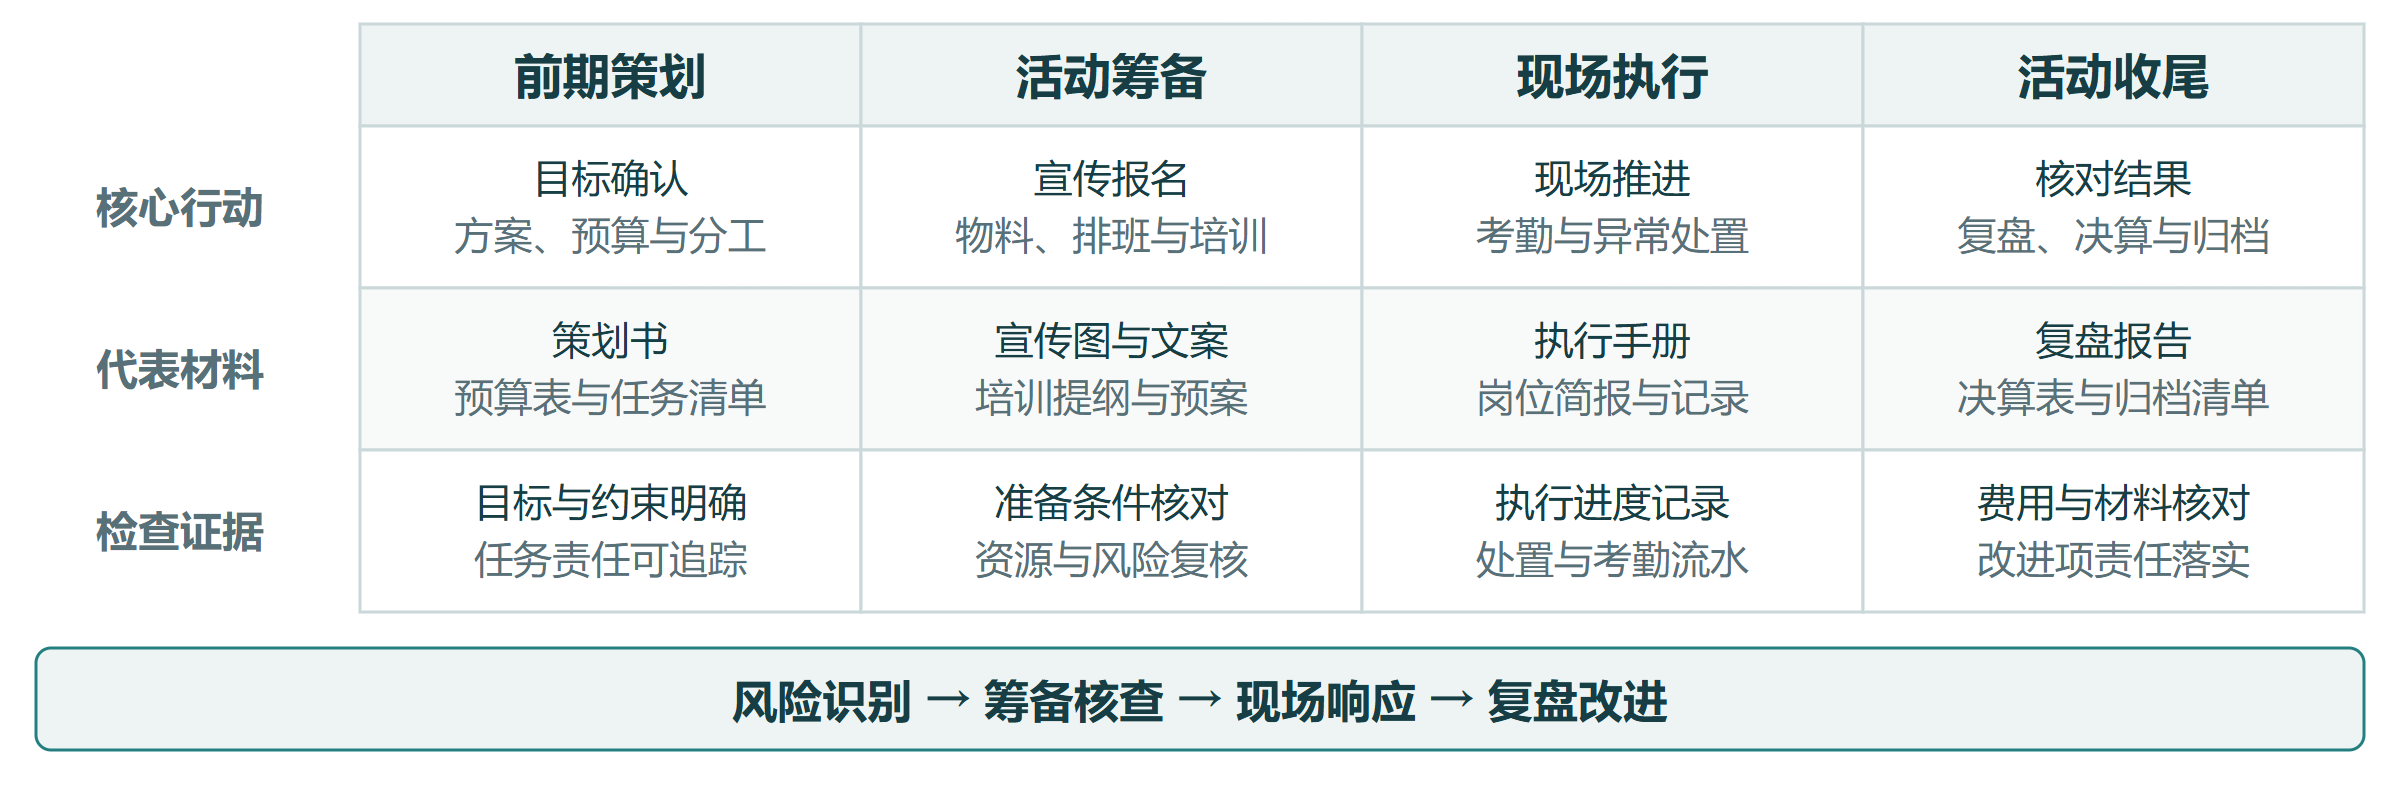
\includegraphics[width=\textwidth]{lifecycle-controls.png}
\caption{全周期行动、材料与检查证据的对应关系}
\label{fig:lifecycle}
\end{figure}

建设范围包括项目管理、任务排期、人员排班、资源与风险台账、材料生产、知识素材、卡片工作流，以及邀请协作和考勤。验证时检查阶段衔接、材料内容与格式、风险响应规则，并核对协作权限、保存状态和版本冲突处理。

项目以校园科技文化节贯通需求分析、功能展示和成果检查。活动信息、任务和产出可以按项目配置，使同一工作台能够复用于运动会、迎新、竞赛等活动。

\section{需求分析与结构化分解}
\subsection{全周期任务结构}
任务分解先确定分类维度，再逐层展开。项目采用 MECE 的过程时间法，将活动划分为策划、筹备、执行和收尾四阶段；各阶段围绕应完成的行动构建逻辑树，形成图\ref{fig:tree}所示的任务结构。\source{3}这一划分为排期、阶段检查和成果归档提供统一顺序。

\begin{figure}[H]\centering
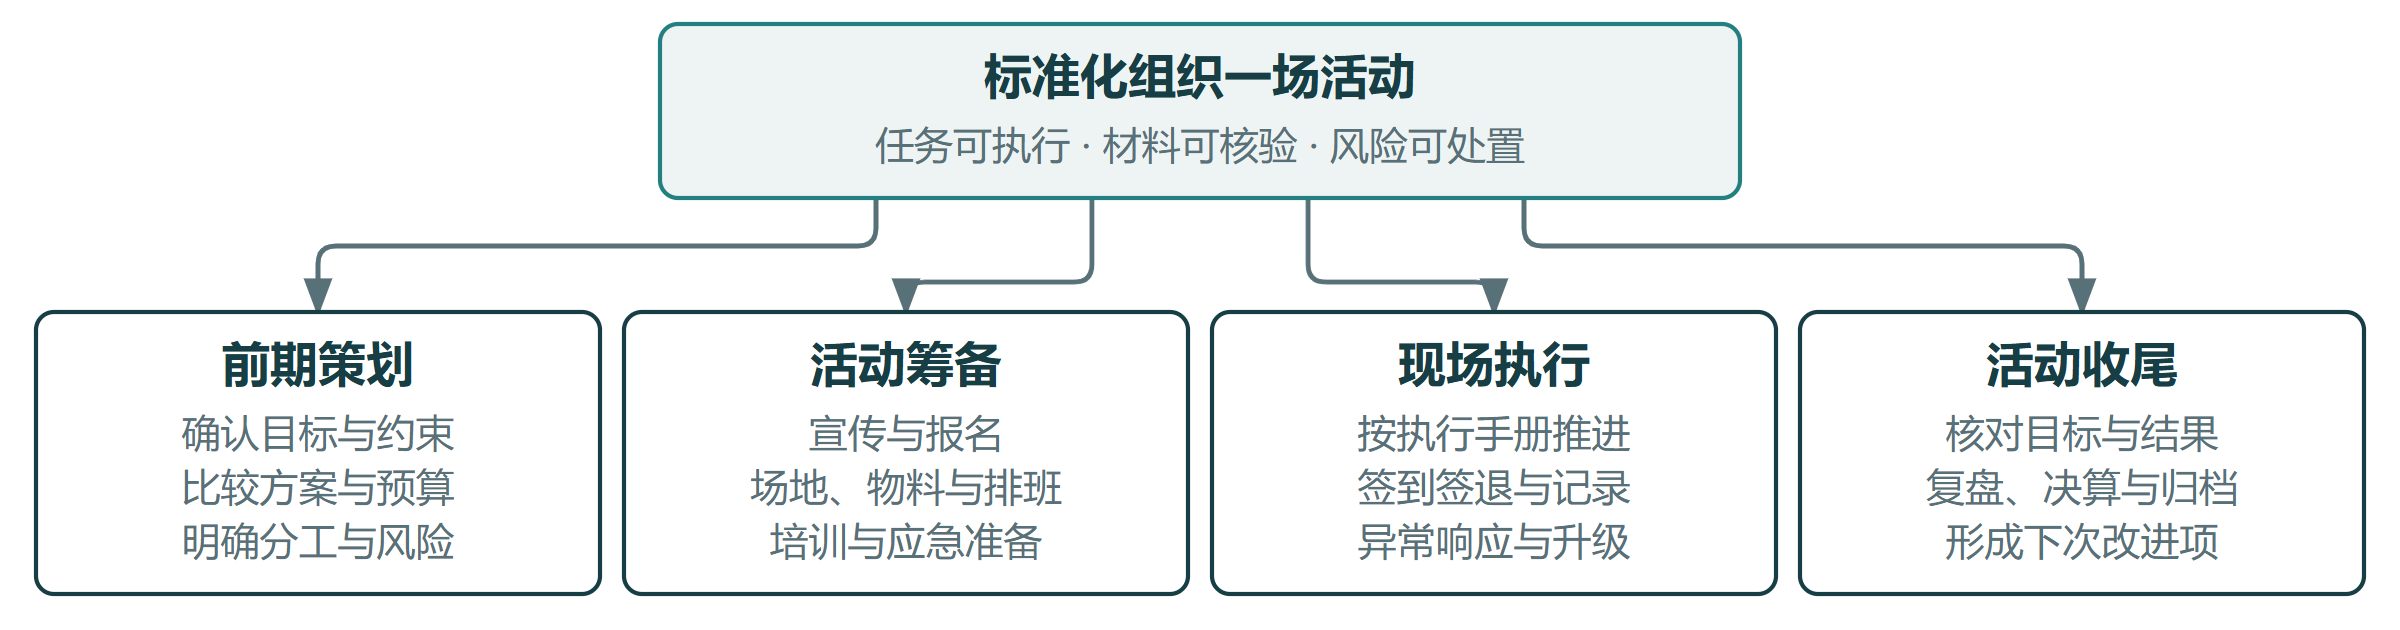
\includegraphics[width=\textwidth]{activity-tree.png}
\caption{按过程时间法构建的活动方案树}
\label{fig:tree}
\end{figure}

MECE 在此用于检查任务边界和覆盖范围。每项任务确定主要所属阶段，跨阶段事项拆为可验收节点，再以依赖关系连接。例如场地落实、布置和现场检查分属不同节点，各自具有完成条件。分解持续到“有人负责、有明确动作、有完成证据”，同时核对决算、物料回收和归档等收尾事项是否齐全。

逻辑树明确“有哪些工作”，5W2H 进一步明确“怎样把工作做成”。项目将内容、目的、人员、时间、地点、方法和资源需求转化为任务字段与核验要求，见表\ref{tab:5w2h}。\source{3}

\begin{table}[H]\centering\small
\caption{5W2H 与工作台数据、操作的对应关系}
\label{tab:5w2h}
\begin{tabularx}{\textwidth}{L{2.5cm}Y}
\toprule
任务维度 & 数据位置与核验方式 \\
\midrule
What / Why & 写明任务内容及其服务的活动目标，确定应交付的成果。 \\
Who & 记录实名责任人，关联人员名册与执行班次，区分岗位要求和实际人员。 \\
When / Where & 明确活动日期、任务期限、执行地点和备用安排，缺项保留待确认。 \\
How & 用任务依赖、执行手册和检查点说明操作步骤及完成条件。 \\
How much & 关联人数、预算和资源需求，核对可用数量、已安排数量及费用明细。 \\
\bottomrule
\end{tabularx}
\end{table}

以“完成场地准备”为例，任务需明确由谁在何时完成布置、使用哪些设备与物料、按什么清单检查，以及提交什么证明材料。这样，任务名称能够转化为可执行安排，后续交付与验收也有共同依据。未确认的事实由组织者补充，AI依据已有信息辅助展开。

\subsection{功能、材料与风险的对应关系}
时间阶段回答“何时推进”，管理对象回答“需要统筹什么”。工作台围绕同一项目关联任务、人员、资源、材料和风险：任务驱动行动，人员与资源保障实施，材料承载成果，风险规定预防和应急要求。表\ref{tab:trace}将建设目标对应到功能与检查证据，形成从需求到验收的追踪关系。

\begin{table}[H]\centering\small
\caption{核心需求追踪表}
\label{tab:trace}
\begin{tabularx}{\textwidth}{L{2.6cm}Y Y}
\toprule
需求 & 对应能力 & 应检查的证据 \\
\midrule
全周期管控 & 任务分解、排期、人员班次与阶段检查 & 四阶段任务、责任、依赖及交付记录 \\
详尽中间产物 & 产出模板、参考表填值、编辑与导出 & 策划、宣传、执行及收尾文件的内容与版本 \\
风险识别与预案 & 风险台账、矩阵、处置卡与演练 & 评分依据、触发信号、处置动作和升级责任 \\
协作与资料复用 & 账号名册、邀请权限、资料引用与卡片依赖 & 人员资格、共享版本、来源及引用内容 \\
\bottomrule
\end{tabularx}
\end{table}

风险管理同样按这一关系展开。风险先关联发生阶段和受影响任务，再依据可能性与影响评分，明确预防、响应及升级安排；检查时核对触发信号和责任人，演练后修订处置卡。风险评分用于确定关注顺序，行动规则则用于指导具体处置。

材料依据分为活动事实与参考资料。名称、时间、地点、人数及预算由项目信息统一维护；流程、规范与经验进入知识素材库，注明来源、适用范围和核验状态。图片与链接通过人工填写的说明或摘要参与引用，资料修改后重新确认。\source{6}这一组织方式为材料复用和事实核对提供依据。

\subsection{AI 输入结构与过程闭环}
AI 材料生产从明确输入要求开始。项目采用 ALIGN，将目标（Aim）、深度（Level）、依据（Input）、规则（Guide）和成果（Need）写入技能包。\source{4}以策划书为例，目标是支撑活动组织，深度应覆盖任务与责任，依据来自项目信息和选定资料，规则要求未确认事实保留待确认，成果规定章节、表格和交付形式。图\ref{fig:align}展示这些要求如何共同约束生成。

\begin{figure}[H]\centering
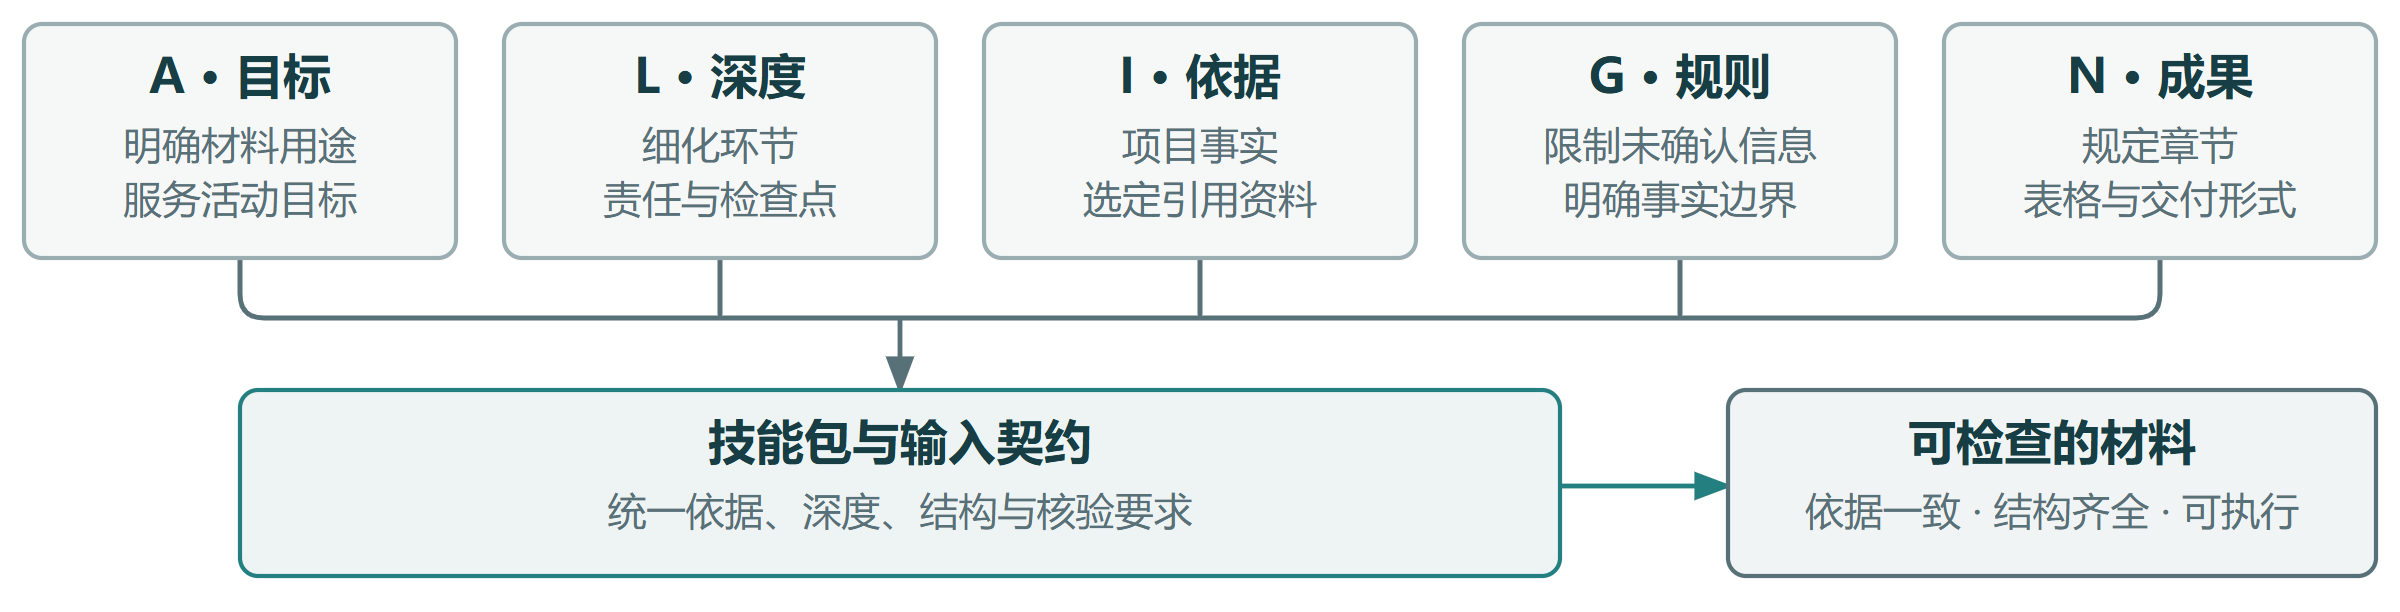
\includegraphics[width=\textwidth]{align-inputs.png}
\caption{ALIGN 输入结构与材料生成要求}
\label{fig:align}
\end{figure}

任务清单等边界明确的产出采用 RTGO，规定角色、任务、目标和输出。\source{4}例如以活动筹备助手为角色，要求依据已确认方案拆解任务，目标是责任和交付清楚，输出包含阶段、期限、负责人、成果及前置依赖。卡片工作流把经确认的上游结果传入下游，使任务清单、宣传材料和执行手册沿同一依据展开。

PDCA 将这些成果纳入实际推进过程：计划阶段明确目标、任务与预案；执行阶段完成筹备、材料和现场操作；检查阶段依据交付、考勤与演练记录核对偏差；改进阶段修订安排并留下处理记录。\source{3}图\ref{fig:pdca}说明这一循环如何连接计划与反馈。事实确认、资源协调和验收判断由使用者承担，AI提供整理、展开和修订辅助。

\begin{figure}[H]\centering
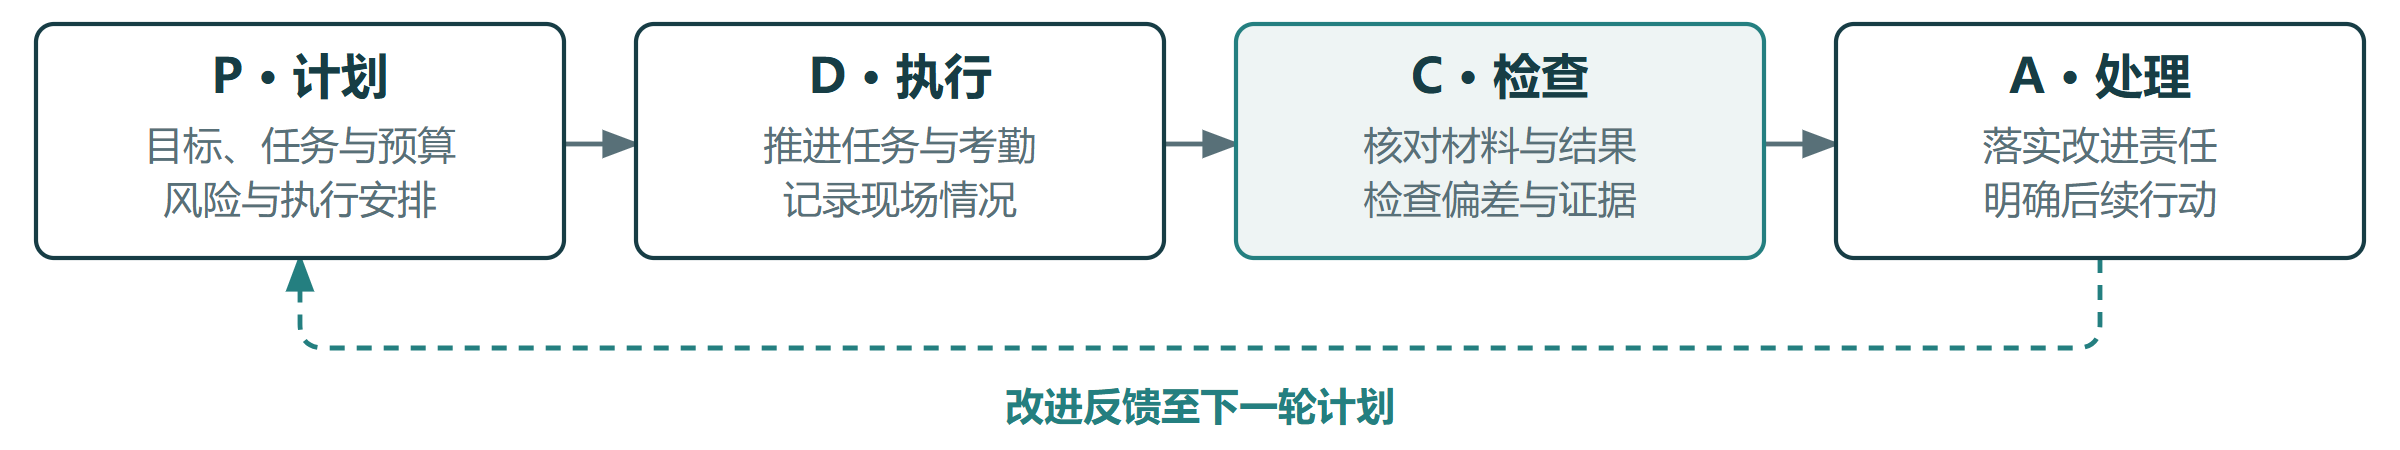
\includegraphics[width=\textwidth]{pdca-cycle.png}
\caption{PDCA 与活动管控的反馈闭环}
\label{fig:pdca}
\end{figure}

\section{方案比较与总体设计}
\subsection{候选路线比较与选择}
技术路线围绕建设目标比较：能否贯通四阶段，能否形成可编辑的过程材料，能否关联风险与应急行动。在此基础上，进一步考虑实现难度、AI 输入控制、协作方式和运行维护。项目比较 AI 对话配合文档表格、低代码或在线协作平台、自建浏览器工作台三类路线，见表\ref{tab:routes}。

\begin{table}[H]\centering\footnotesize
\caption{三类技术路线的适配性比较}
\label{tab:routes}
\begin{tabularx}{\textwidth}{L{2.25cm}Y Y Y}
\toprule
维度 & AI对话与文档表格 & 低代码或协作平台 & 自建工作台 \\
\midrule
实现难度 & 上手较快，关联与版本靠人工组织 & 取决于现成能力及配置工作 & 需开发与测试，已有原型基础 \\
全周期关联 & 通过目录、表格及规则连接 & 借助关联表、流程和权限配置 & 按项目连接任务、人员、材料与风险 \\
材料生产 & 文档便于修改，需统一信息口径 & 模板及导出取决于平台支持 & 支持模板、参考表、编辑与文件导出 \\
AI 输入控制 & 逐次提供上下文和输出要求 & 取决于接口与工作流能力 & 配置技能包、资料引用与卡片依赖 \\
协作与运行 & 可用在线文档，跨成果需整合 & 需核对账号、权限及服务条件 & 邀请共享与冲突保护由运行服务支持 \\
\bottomrule
\end{tabularx}

\end{table}

比较采用定性判断，逐项说明各路线的适配条件。综合全周期关联、材料生产与 AI 输入控制需求，以及已有原型基础，项目选择自建工作台，使任务分解、资料引用和交付验收能够直接落实到数据与操作规则。

随后运用 SWOT，从内部能力与外部环境检视实施条件，见表\ref{tab:swot}。\source{3}分析结果用于确定运行、保存和演示安排。

\begin{table}[H]\centering\small
\caption{自建工作台路线的 SWOT 分析}
\label{tab:swot}
\begin{tabularx}{\textwidth}{Y Y}
\toprule
内部优势 S & 内部劣势 W \\
\midrule
已有四阶段管理、材料导出和风险机制；技能包与卡片可按任务配置。 & 共享采用版本快照，冲突需人工处理；文件存储按单进程运行，存档需配套备份。 \\
\midrule
外部机会 O & 外部威胁 T \\
\midrule
不同活动具有相近的组织环节，任务与材料结构具备复用条件。 & 网络及外部 AI 服务状态影响在线调用；生成内容可能缺乏事实依据。 \\
\bottomrule
\end{tabularx}
\end{table}

据此，方案以全周期任务和材料关联发挥可配置优势，采用项目包与服务数据备份保存成果，保留共享冲突恢复流程，并用已核验材料支撑本机演示。AI 输入限定依据范围，输出经过人工确认后进入交付。路线选择与运行安排由同一组目标和约束支撑。

\subsection{系统架构与数据关联}
系统采用原生 JavaScript 前端与 Node 服务，接入 DeepSeek 文字生成和 GPT-image2 图像生成。\source{5}浏览器承担项目操作、可视化与材料编辑，手机入口支持报名、任务和考勤，服务端处理账号、共享、排班、交付与 AI 请求。主要组件和数据流见图\ref{fig:architecture}。

\begin{figure}[H]\centering
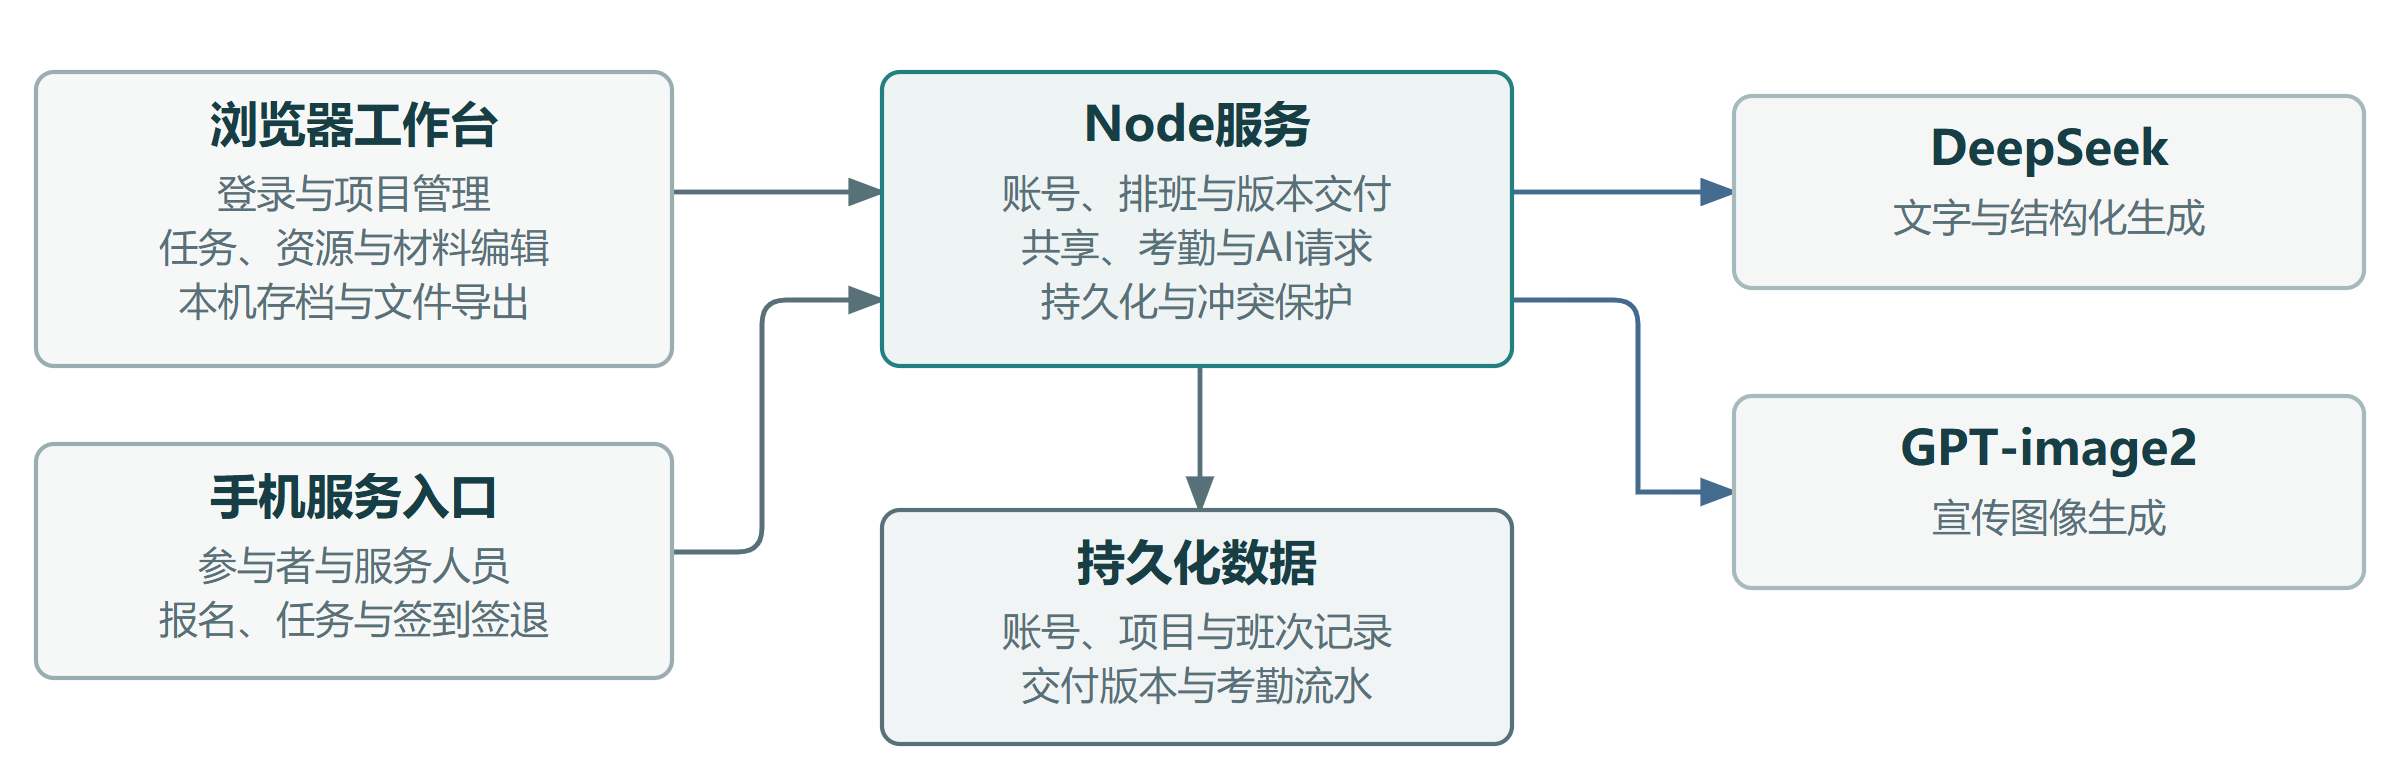
\includegraphics[width=\textwidth]{system-architecture.png}
\caption{系统架构与主要数据流}
\label{fig:architecture}
\end{figure}

数据关系以项目为中心展开。活动事实统一任务与材料的基本口径；任务关联阶段、责任人、期限、依赖和产出；人员名册连接岗位、班次与考勤；风险连接任务与处置动作。执行记录进入检查和复盘，形成从计划到结果的追踪链条。

材料交付通过编号与版本连接任务验收。责任人提交经确认的材料版本，组织者据此检查成果；交付保存独立快照，后续编辑保持既有验收依据可追溯。\source{5}这一设计把“谁完成、完成什么、依据哪个版本”落实为具体关联，支撑 5W2H 的责任要求和 PDCA 的检查环节。

协作按邀请权限和版本快照同步，交付与验收核对账号及项目人员资格。只读访问用于查看，编辑保存核对版本，冲突时保留本机草稿供处理。账号、共享项目、班次和考勤由单个 Node 进程保存到文件目录，浏览器项目包与服务数据分别备份。\source{5}上述规则共同支撑多人操作、成果留存与过程追踪。

\section{工作台建设与 AI 应用}
工作台以项目为中心，将活动事实、任务、人员、资源、风险与材料放在同一操作空间中。本章沿“进入项目、推进任务、保障执行、形成材料”的顺序展示主要内容，再说明 AI 应用与建设分工。

\subsection{项目管理与全周期管控}
\textbf{项目入口统一活动信息。}登录后先进入项目库，查看、新建、导入或打开项目，也可复制已有项目用于另一场活动。图\ref{fig:ui-projects}展示项目卡片、状态筛选与项目包操作。打开项目后，账号资料自动登记到人员名册，活动名称、日期、地点、人数与预算在项目信息表中统一维护。\source{5}

\begin{figure}[H]\centering
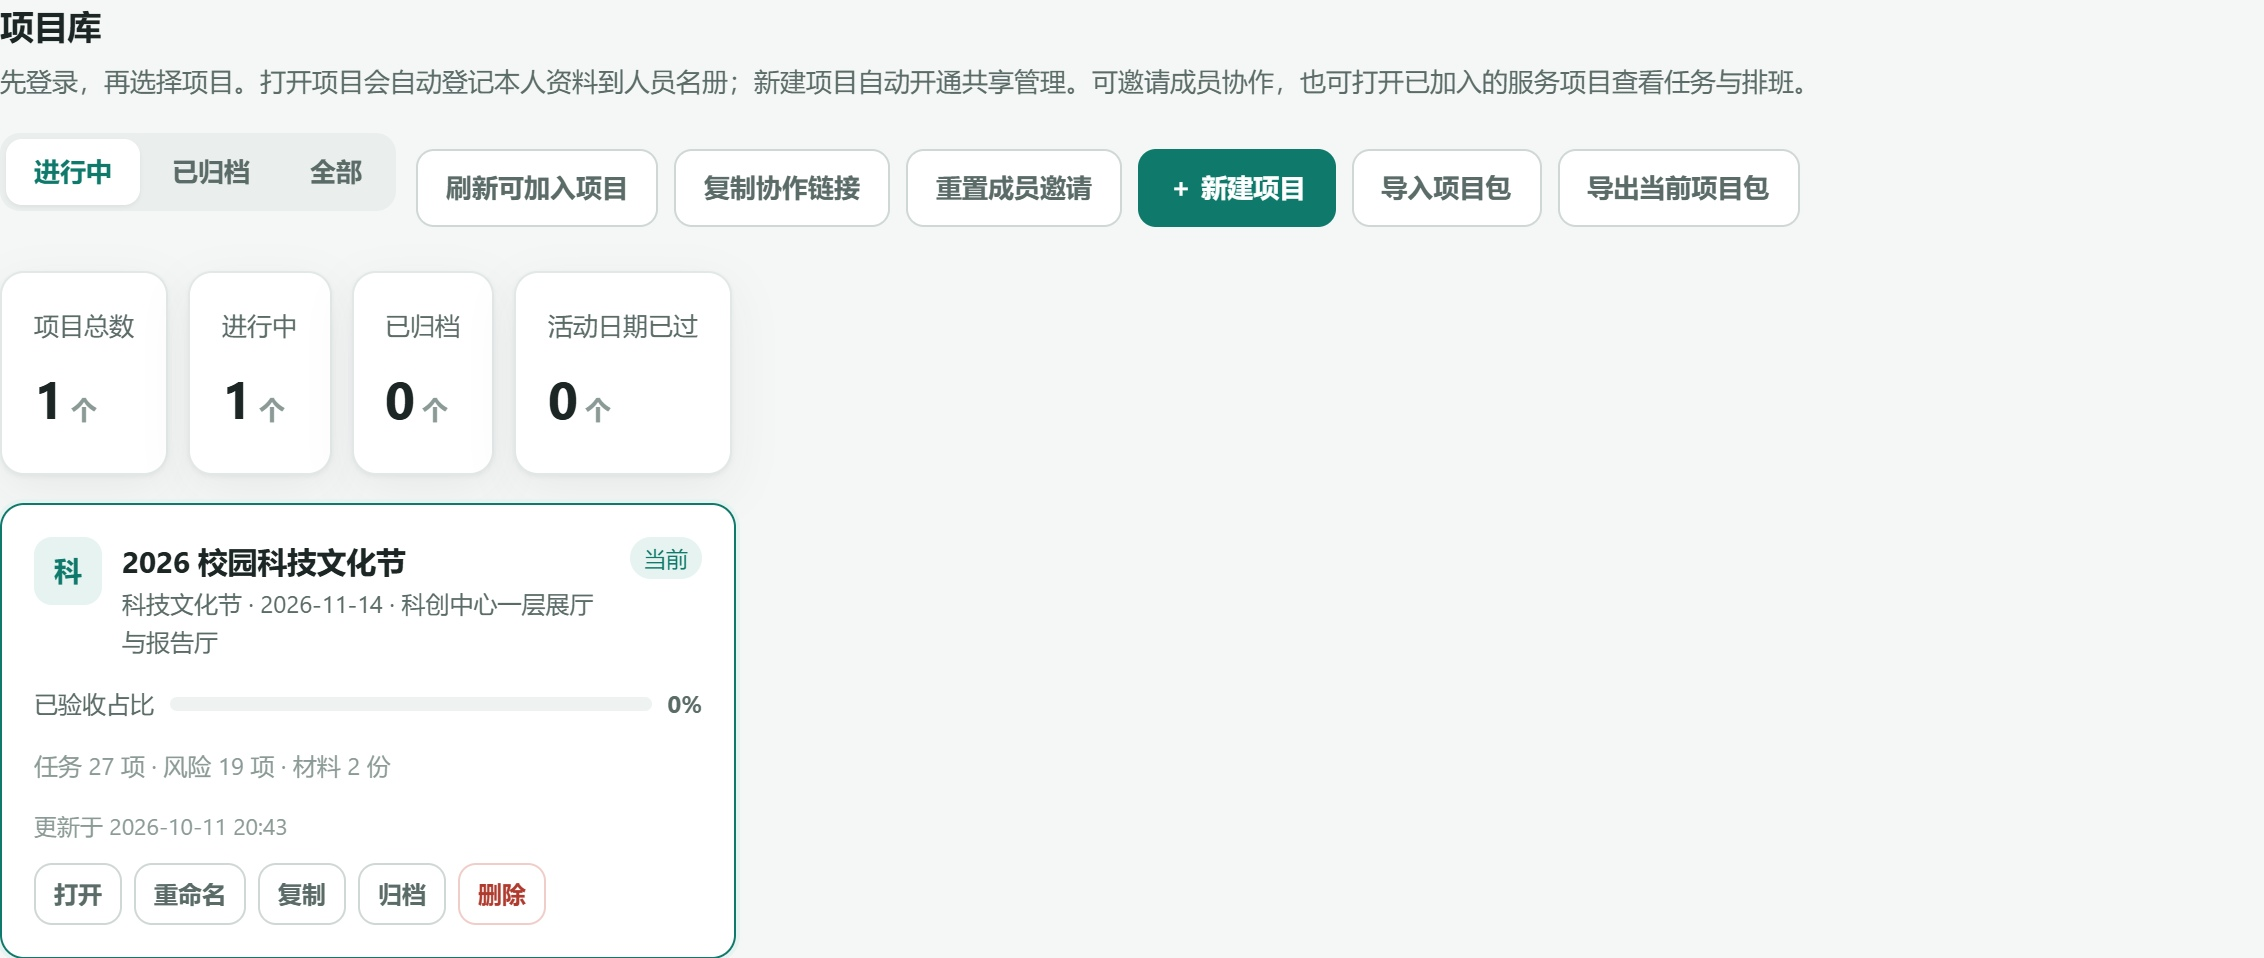
\includegraphics[width=\textwidth]{screenshots/project-entry-d39138e.jpg}
\caption{登录后的项目库与创建、导入、导出入口}
\label{fig:ui-projects}
\end{figure}

全周期操作流程见图\ref{fig:mainflow}。策划、筹备、执行和收尾按时间顺序组织，任务、材料与风险沿阶段关联；阶段检查发现缺项时返回补齐，协作与风险管理贯穿全过程。

\begin{figure}[H]\centering
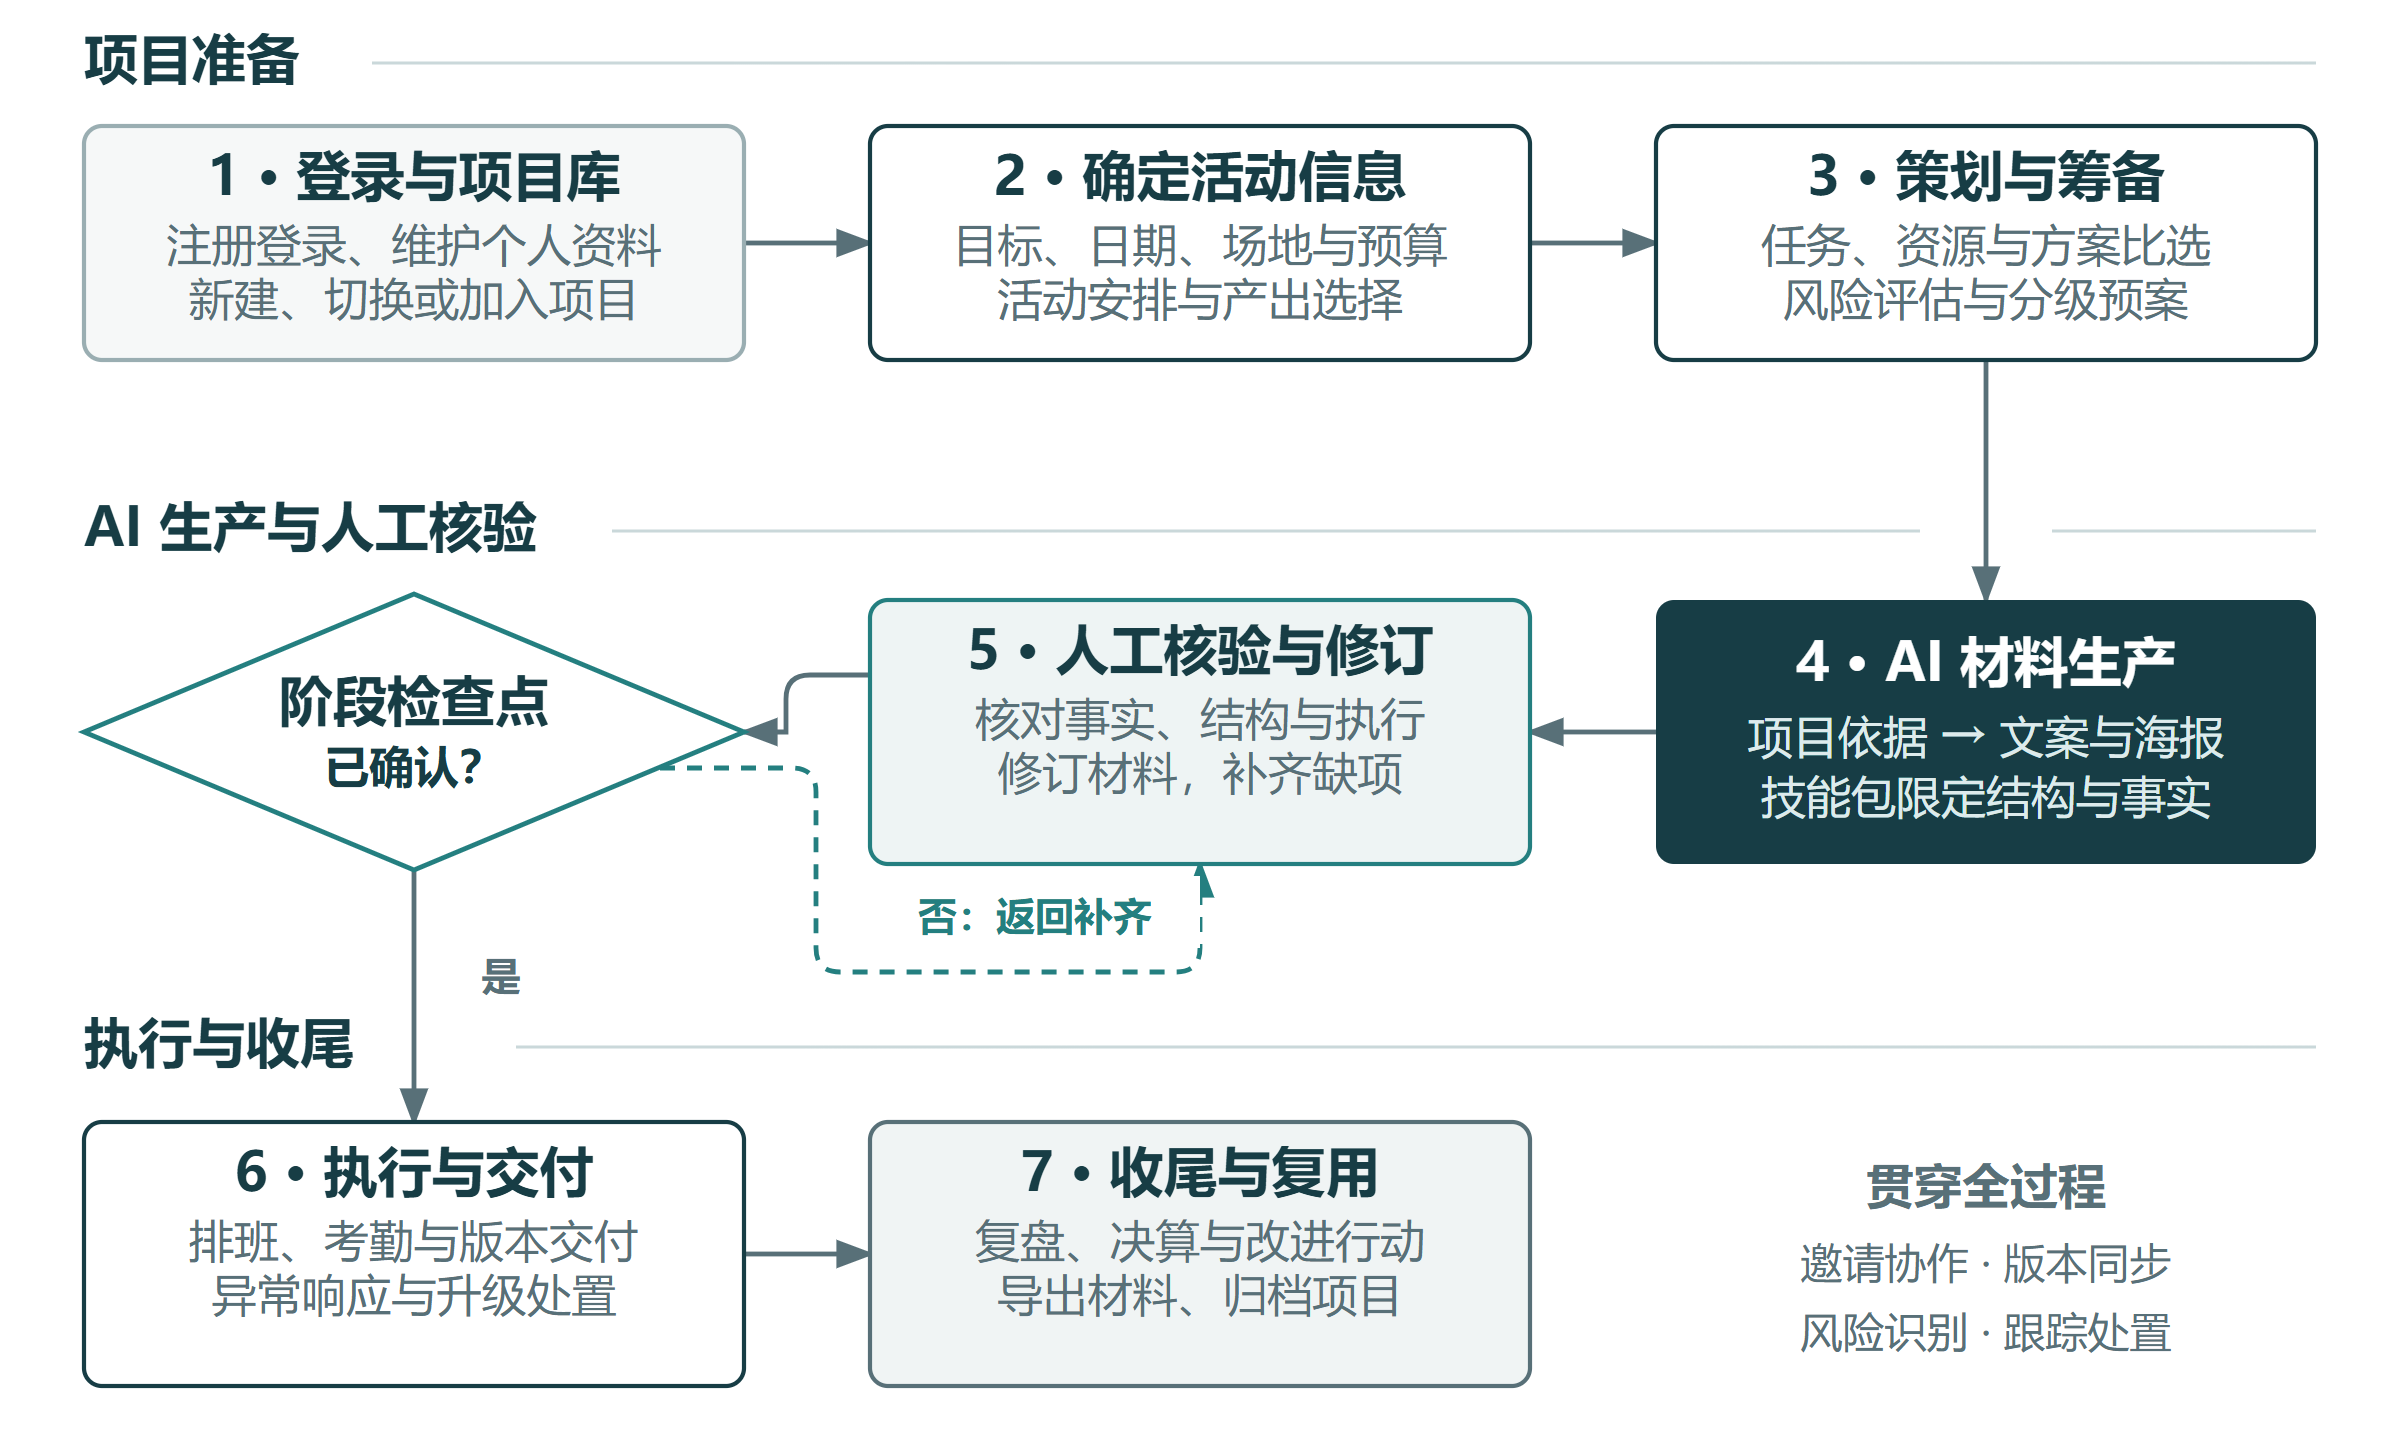
\includegraphics[width=\textwidth]{workbench-main-flow.png}
\caption{工作台主要功能与全周期使用流程}
\label{fig:mainflow}
\end{figure}

\textbf{任务管理把计划转为可执行安排。}总览汇集阶段验收、关键节点与缺口提醒（图\ref{fig:ui-overview}）。任务页提供分解表、甘特与检查点，关联期限、岗位、产出、依赖、实名责任与班次（图\ref{fig:ui-tasks}），将 5W2H 落实到行动与交付。

\begin{figure}[H]\centering
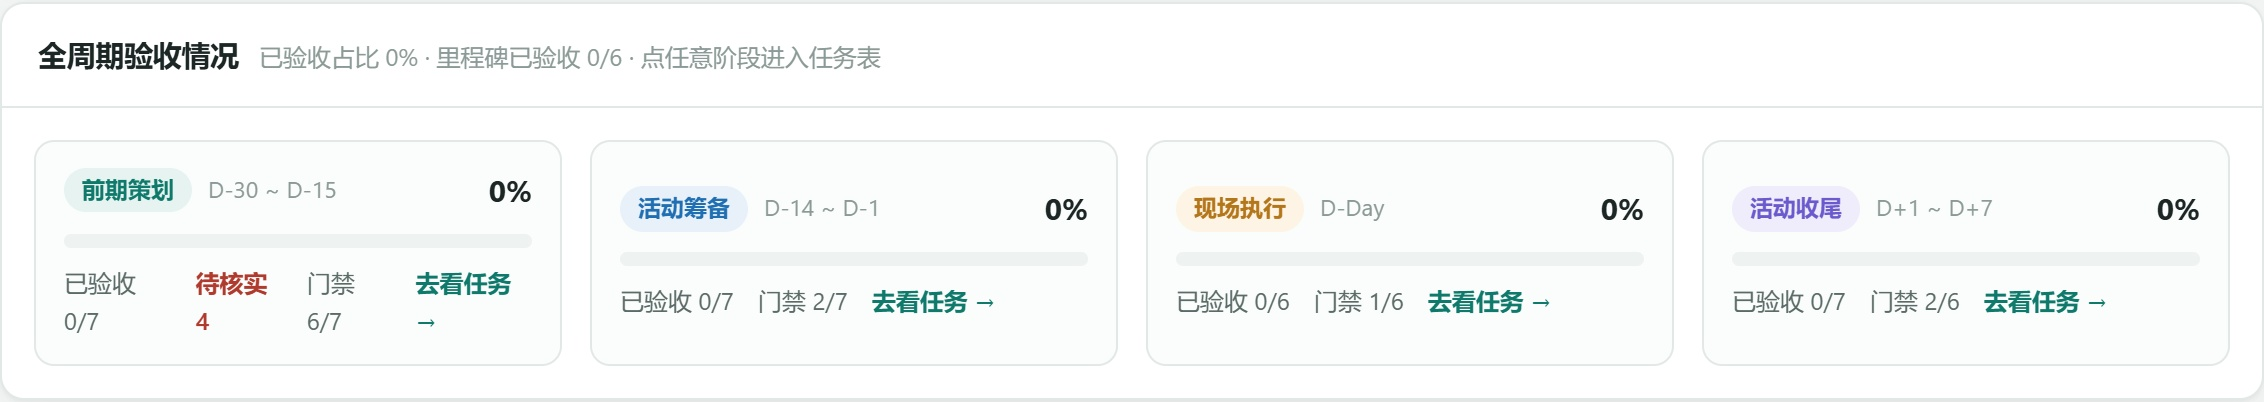
\includegraphics[width=\textwidth]{screenshots/overview-detail.jpg}
\caption{总览中的四阶段验收情况与检查点}
\label{fig:ui-overview}
\end{figure}

\begin{figure}[H]\centering
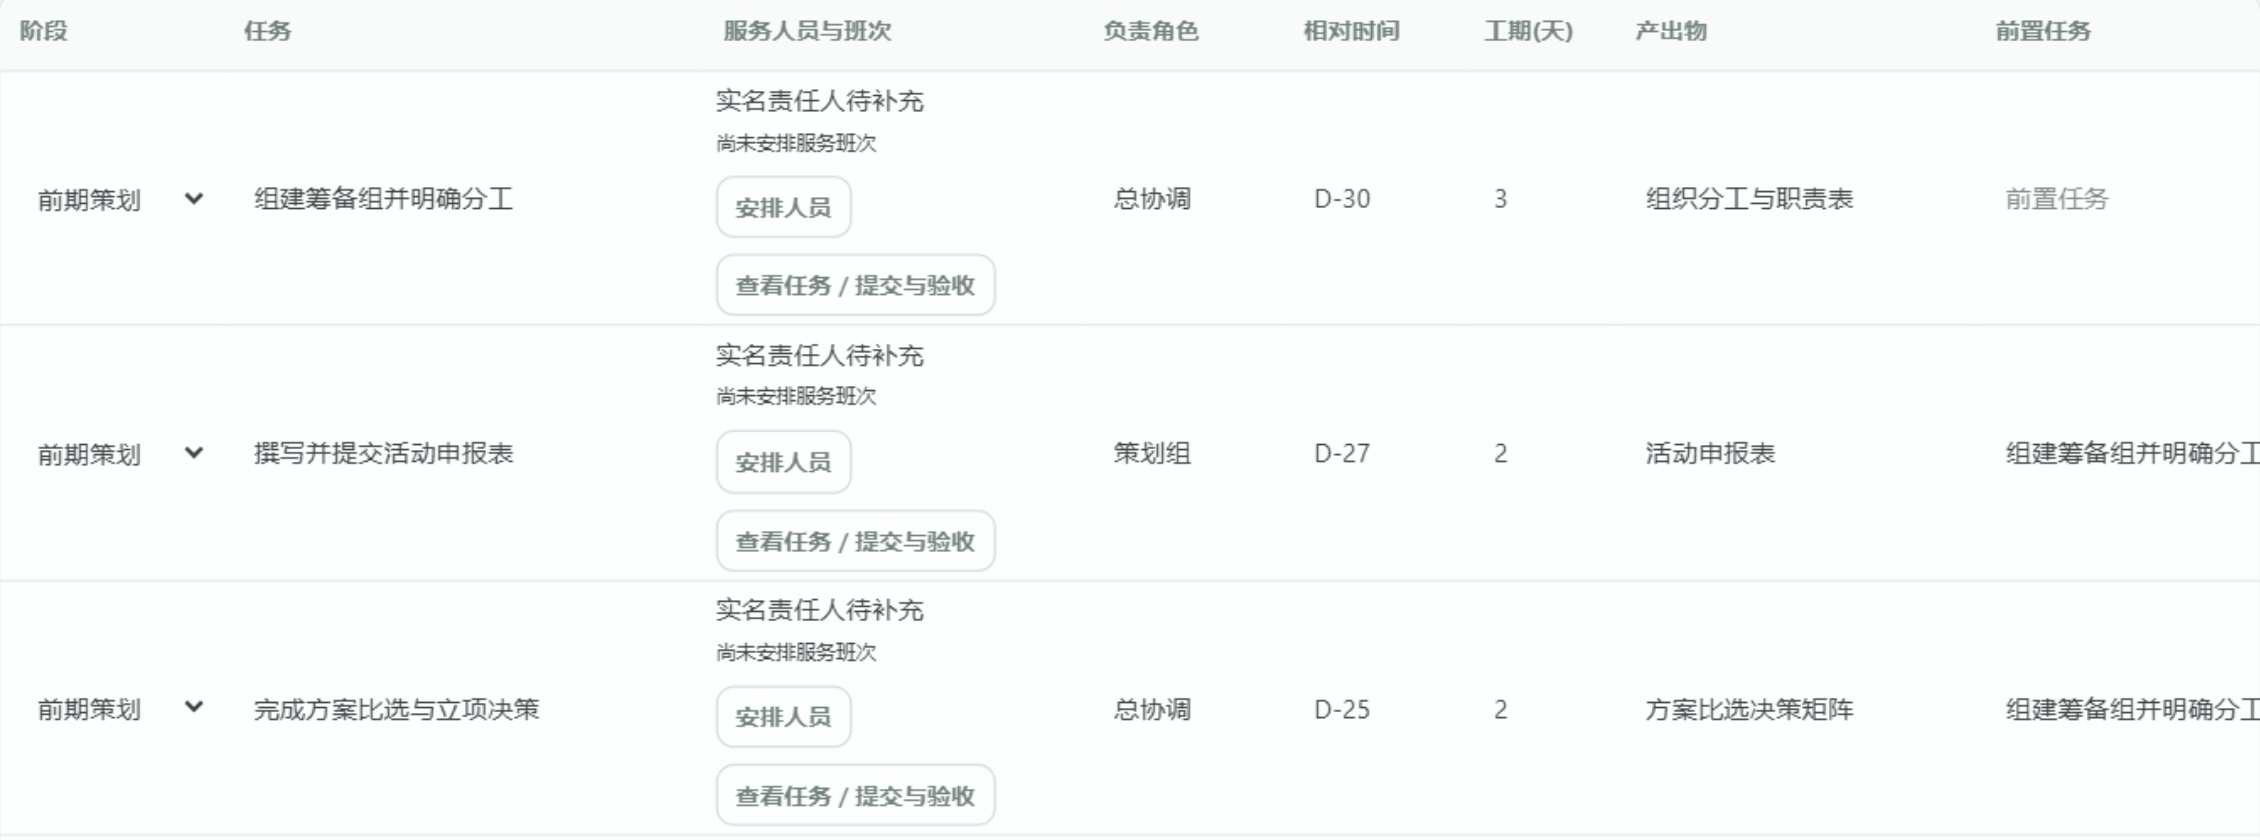
\includegraphics[width=\textwidth]{screenshots/tasks-detail.jpg}
\caption{全周期任务表中的阶段、期限、岗位与交付要求（局部）}
\label{fig:ui-tasks}
\end{figure}

\textbf{人员与资源支撑现场执行。}人员名册集中显示身份、入组状态、技能、可服务时间和班次；负责人确认新成员后，从任务页安排多人轮班。成员在“我的任务”查看岗位要求、签到签退并填写执行报告，报名参与者与服务人员的考勤分别管理。图\ref{fig:ui-personnel}展示负责人及两名演示执行员的名册。\source{5}

\begin{figure}[H]\centering
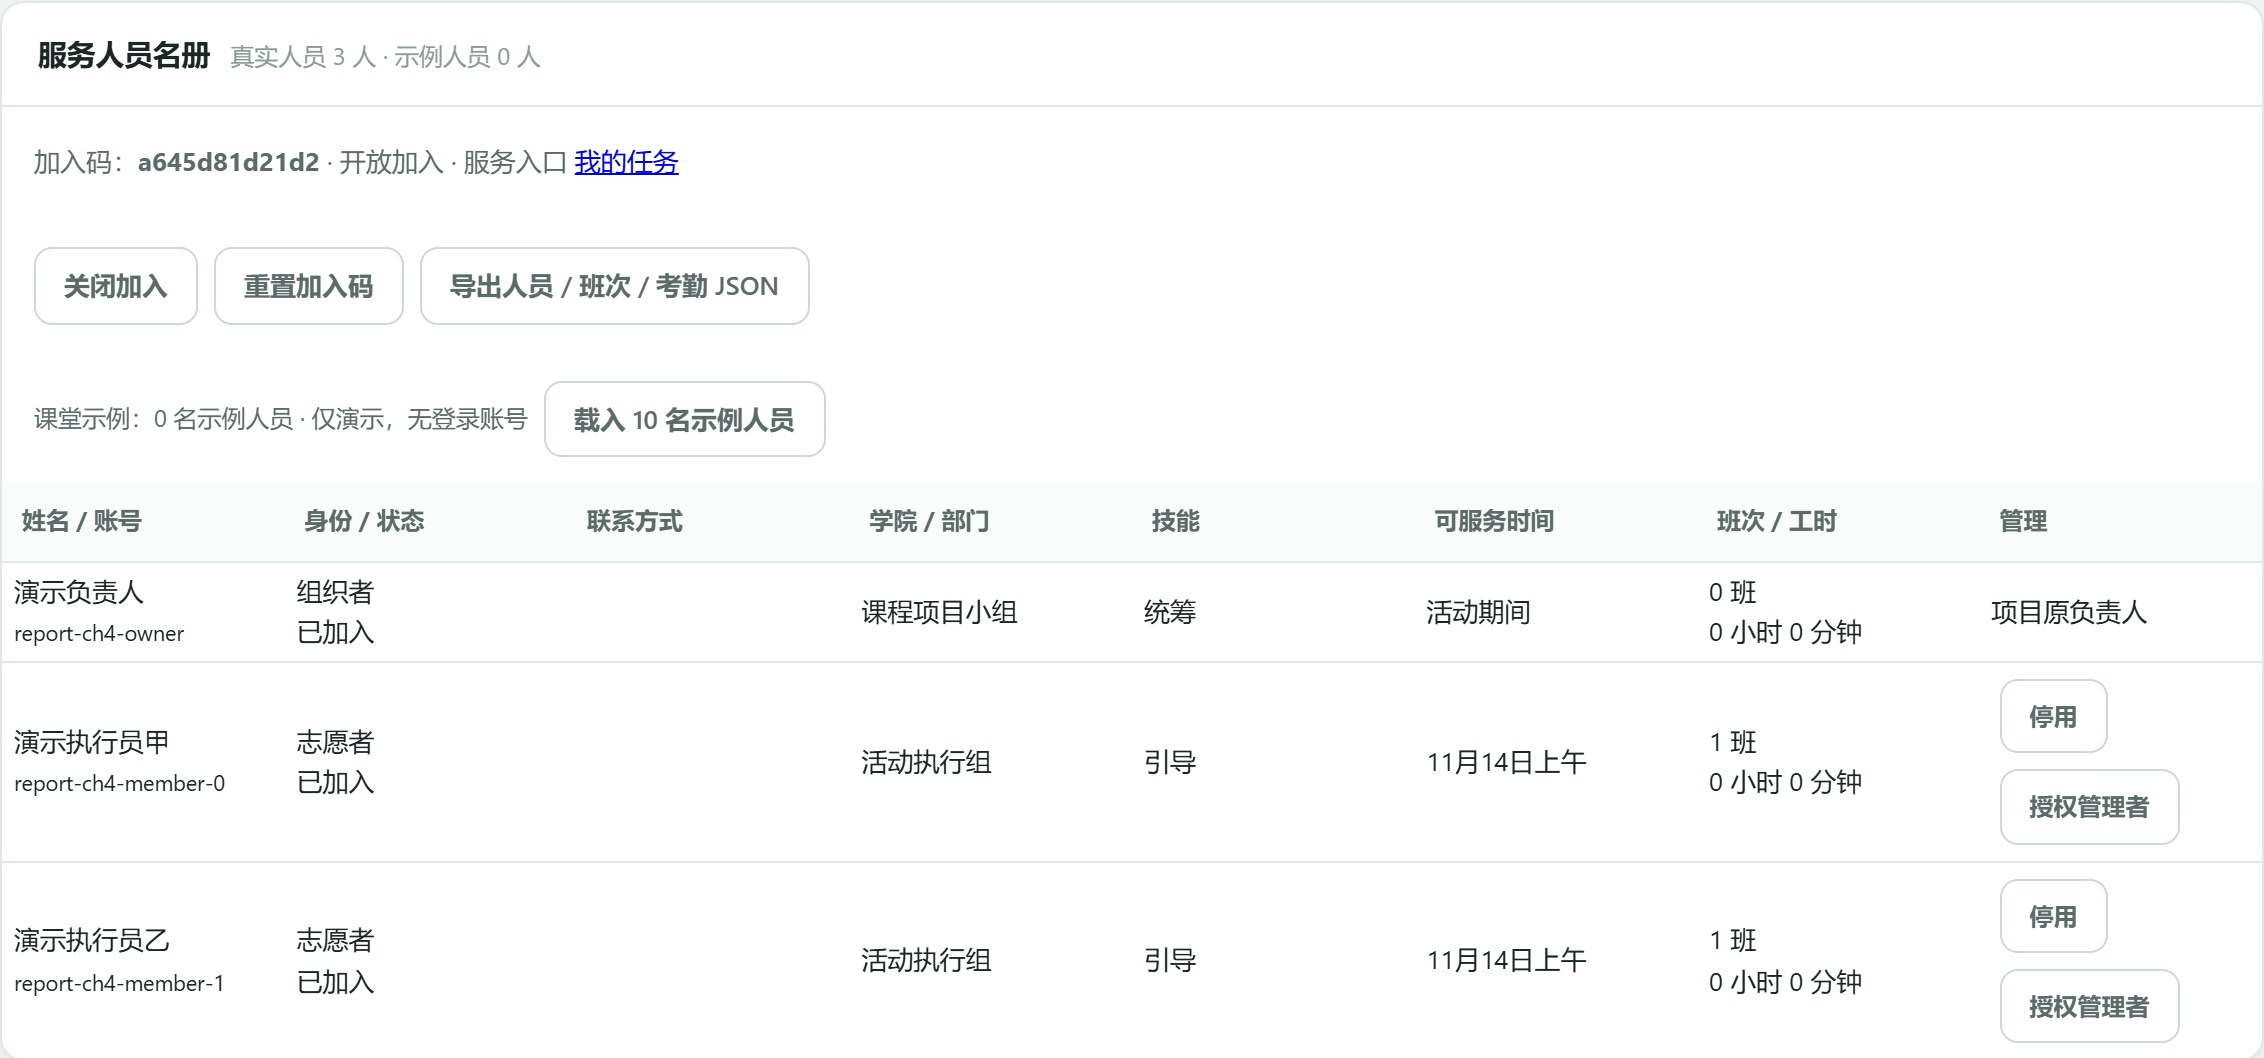
\includegraphics[width=\textwidth]{screenshots/personnel-d39138e.jpg}
\caption{服务人员名册中的身份、技能、可服务时间与班次}
\label{fig:ui-personnel}
\end{figure}

资源台账统一维护物料、设备、场地、车辆与经费，比较库存、借出和计划需求，提示超额占用。图\ref{fig:ui-inventory}呈现示例中的麦克风与运输车辆缺口，组织者据此调整需求或补充资源；物料清单与采购凭证沿同一台账关联，减少多份表格之间的口径差异。

\begin{figure}[H]\centering
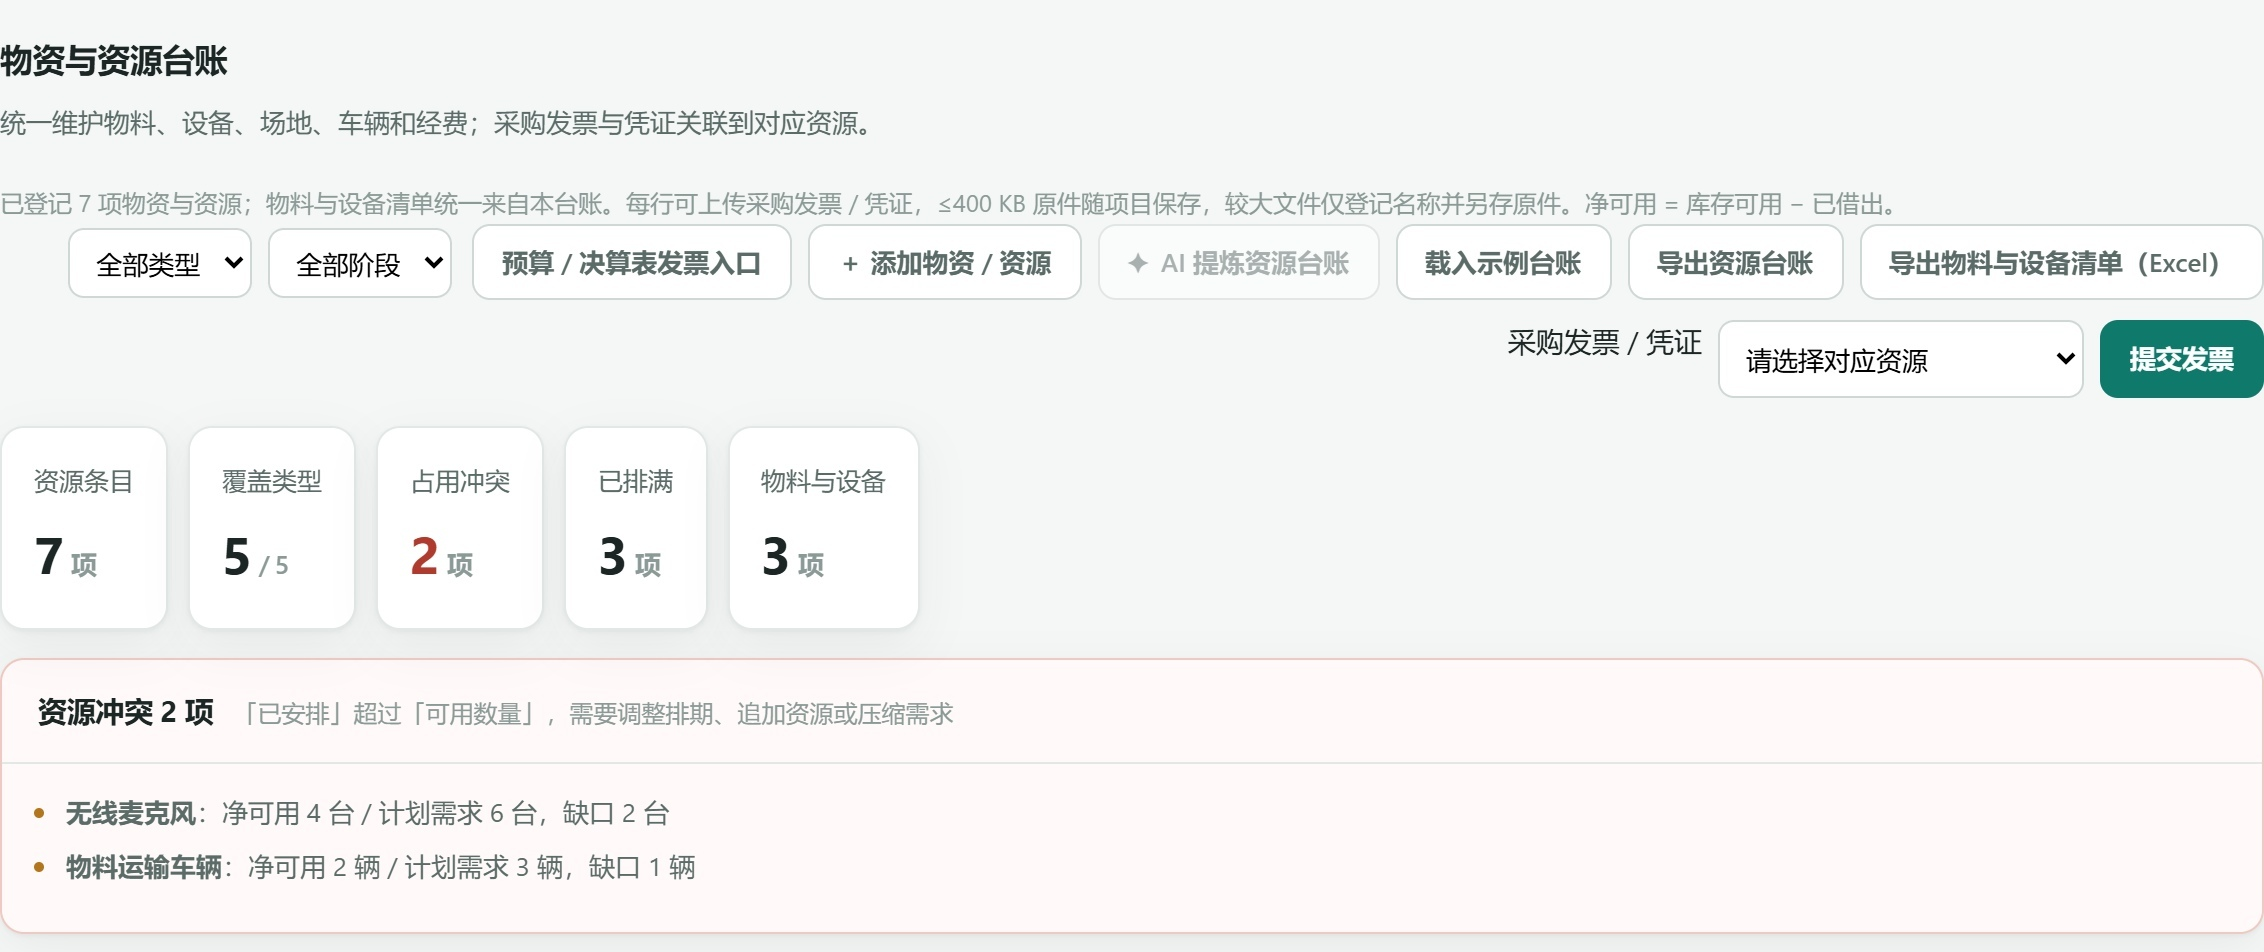
\includegraphics[width=\textwidth]{screenshots/inventory-status-d39138e.jpg}
\caption{资源台账中的库存统计与缺口提示（局部）}
\label{fig:ui-inventory}
\end{figure}

\textbf{风险预案明确异常发生后的行动。}风险台账覆盖十类风险，关联阶段、任务与责任人；处置卡记录可能性、影响及触发信号、预防、响应、升级路径（图\ref{fig:ui-risk}）。评分按可能性与影响乘积分级，规则见图\ref{fig:riskmatrix}；变更演练逐步核对处置动作，并把结论写回台账，形成 PDCA 的检查与修订闭环。\source{8}

\begin{figure}[H]\centering
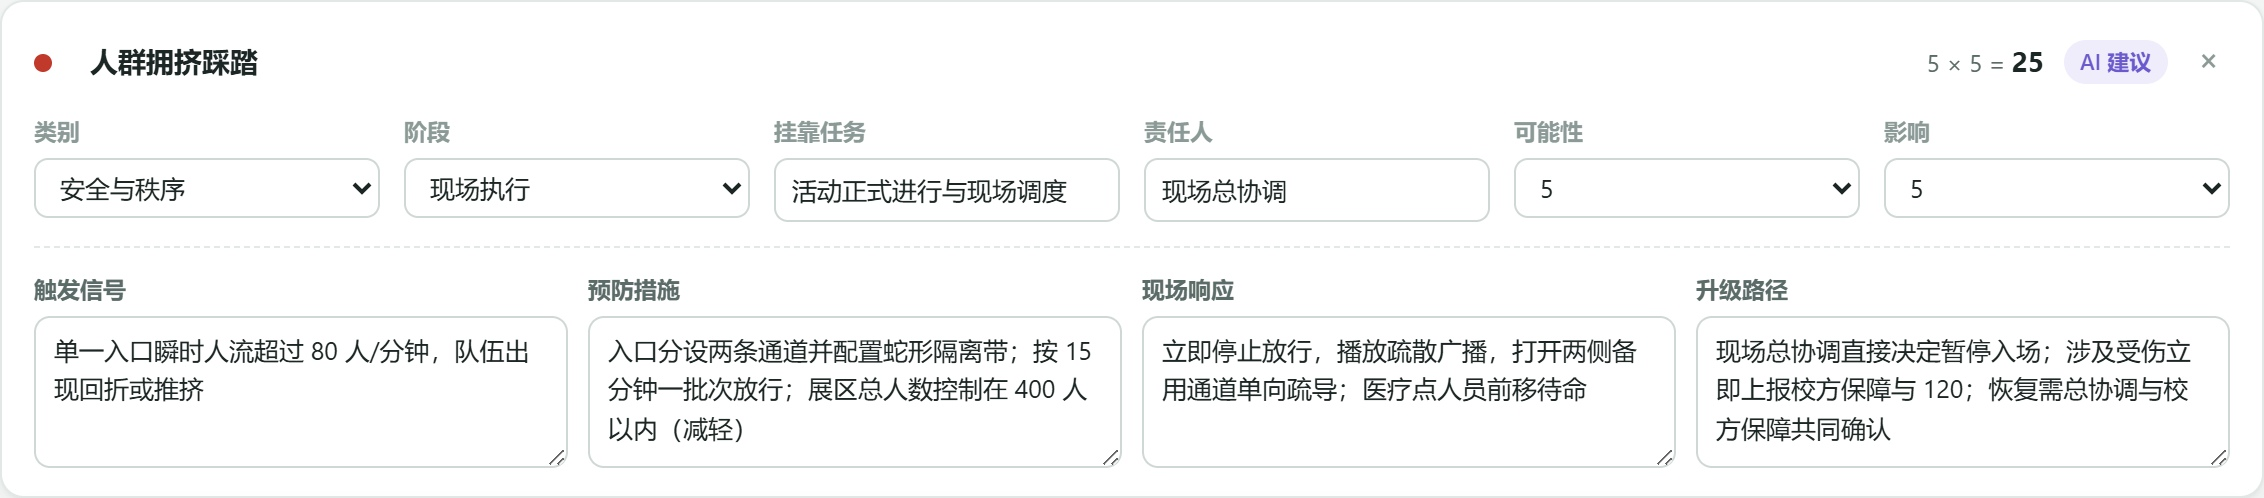
\includegraphics[width=\textwidth]{screenshots/risk-card-d39138e.jpg}
\caption{风险处置卡中的评分、责任与应急四要素}
\label{fig:ui-risk}
\end{figure}

\begin{figure}[H]\centering
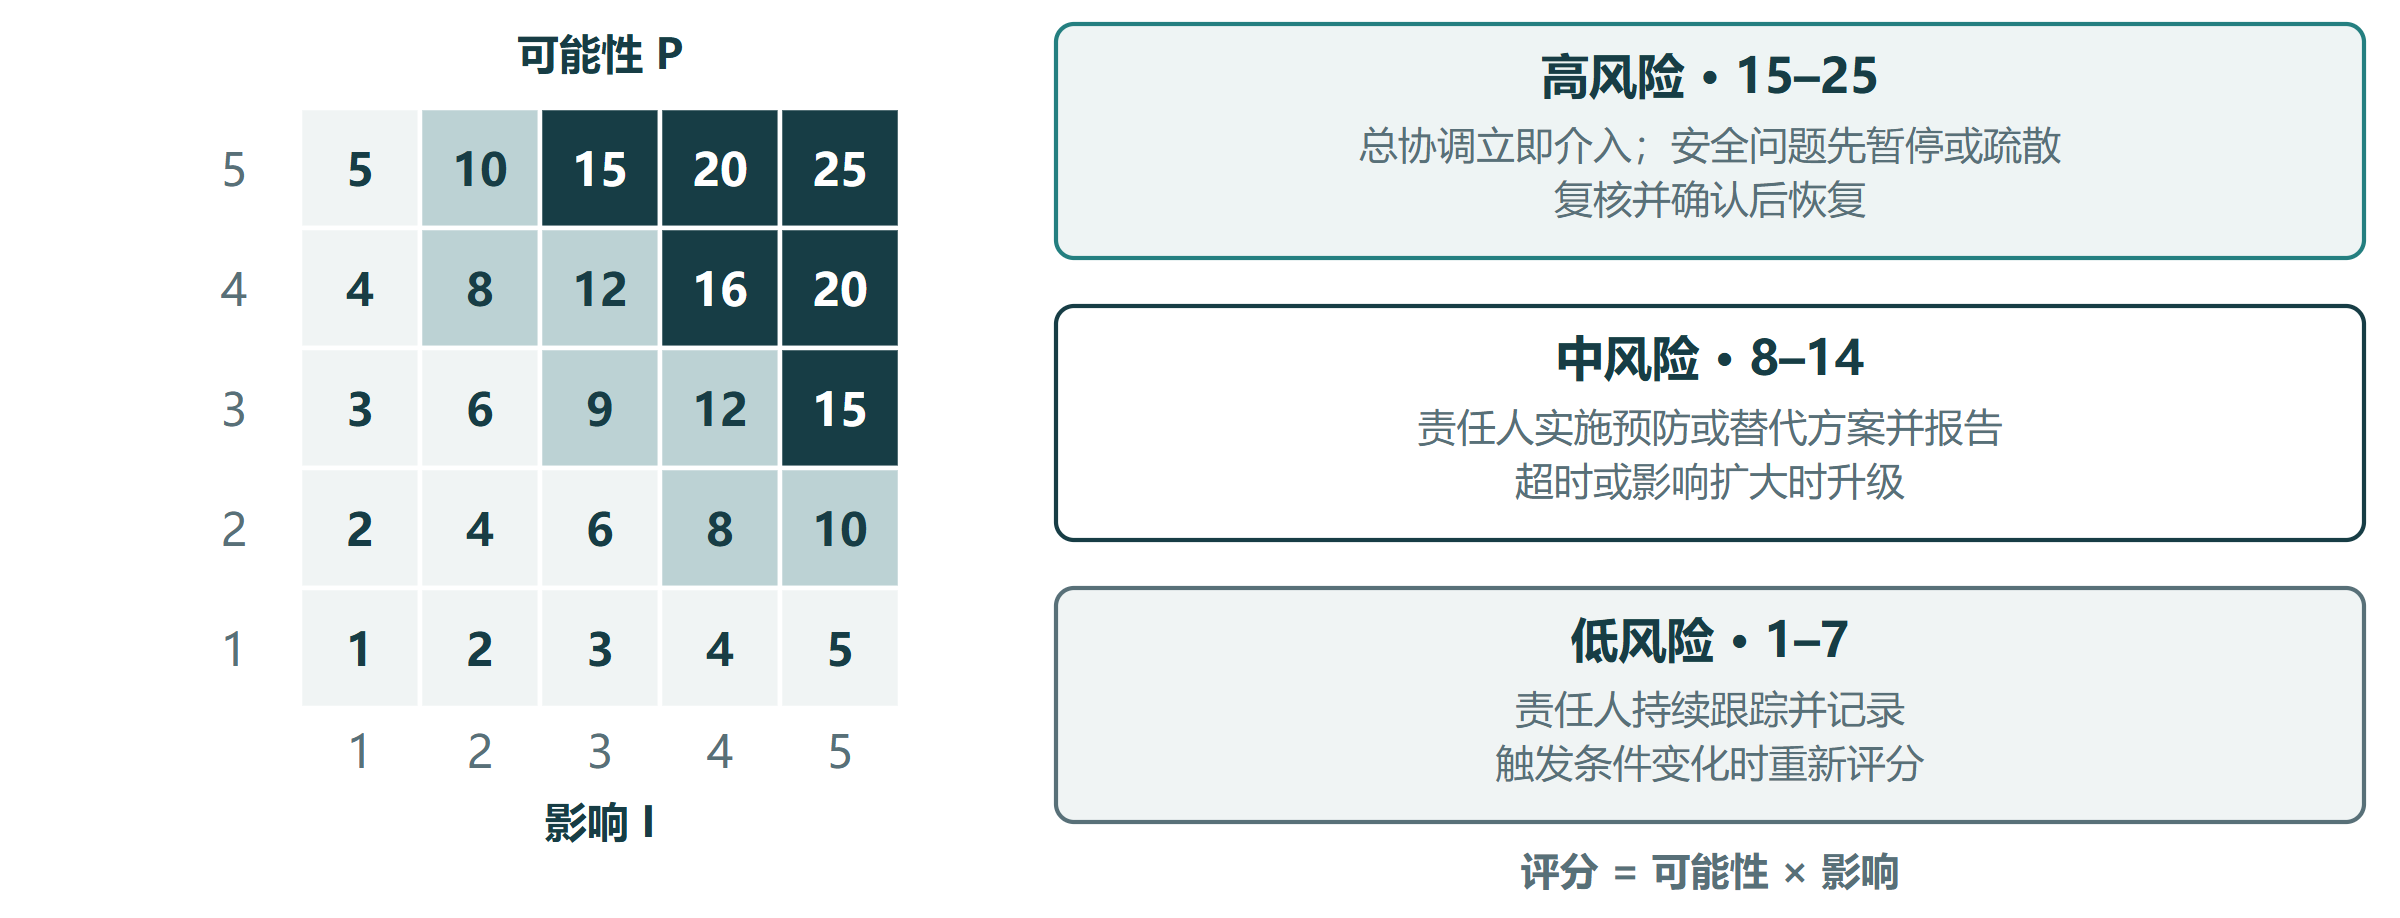
\includegraphics[width=\textwidth]{risk-matrix.png}
\caption{风险评分矩阵与分级响应规则}
\label{fig:riskmatrix}
\end{figure}

邀请链接区分可编辑协作与只读访问；共享保存核对版本，冲突时保留本机草稿。班次报告记录执行过程，任务另行提交实际材料版本，由组织者验收，收尾再导出材料与项目包归档。

\subsection{AI 材料生产与人工核验}
\textbf{资料库为生成提供可复用依据。}知识库保存流程、规范与经验，多模态素材库保存图片、文案及文件。条目登记来源、适用范围、正文和用途，选择“用于 AI 生成”后进入引用内容；知识条目还需核验。图\ref{fig:ui-library}展示主标语的正文与引用开关，使宣传材料沿用同一文案。\source{6}

\begin{figure}[H]\centering
\begin{minipage}[c]{0.36\textwidth}
\centering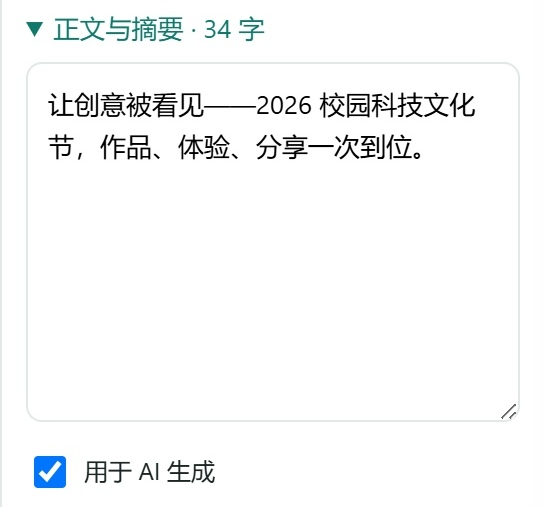
\includegraphics[width=\linewidth]{screenshots/library-reference-d39138e.jpg}
\end{minipage}\hfill
\begin{minipage}[c]{0.59\textwidth}
\small
\textbf{资料从登记到复用}\par\vspace{5pt}
记录来源与用途，区分可引用内容和待确认信息；图片提供画面说明，链接与附件提供人工核对的摘要。\par\vspace{5pt}
生成前预览引用内容，生成后核对事实。已核验资料修改后重新确认，下游材料随依据更新。\par\vspace{5pt}
这将 ALIGN 的“依据与规则”落实到资料选择，控制输入的范围与口径。
\end{minipage}
\caption{素材条目中的正文与 AI 引用开关（局部）}
\label{fig:ui-library}
\end{figure}

\textbf{卡片工作流组织材料之间的依赖。}每张卡片配置技能包、资料来源、上游卡片和追加要求，按依赖顺序运行。图\ref{fig:ui-workflow}展示实际画布中的“活动执行口径 → 参与者通知／现场岗位简报”配置，上游统一事实与安排，下游分别面向参与者和工作人员组织内容。结果可写入过程材料；上游失败跳过下游，循环或失效引用阻止运行，替换时保留原稿。\source{5,6}

\begin{figure}[H]\centering
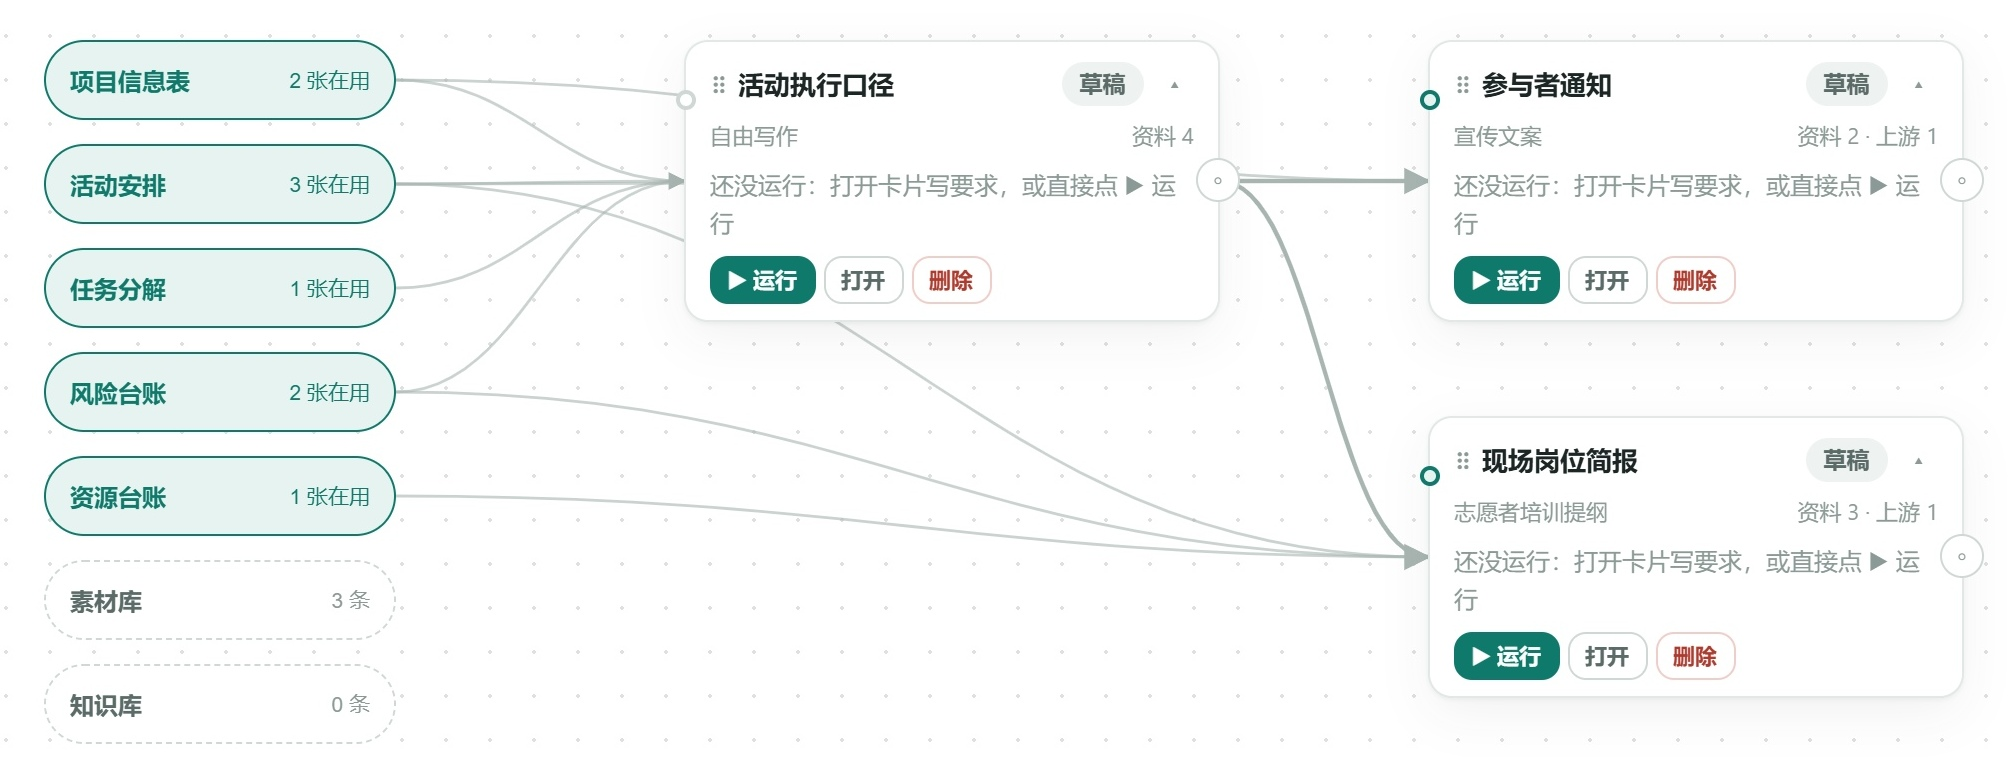
\includegraphics[width=\textwidth]{screenshots/workflow-detail-d39138e.jpg}
\caption{卡片工作流中的资料引用与上下游依赖配置（局部）}
\label{fig:ui-workflow}
\end{figure}

\textbf{过程材料连接生成、编辑与交付。}工作台内置21类产出，支持自定义章节、技能包和参考表。DeepSeek生成文字，GPT-image2生成图片；技能包用 ALIGN、RTGO 明确依据、任务、目标与输出，缺失信息保留待确认。四阶段的代表任务与人工核验重点见表\ref{tab:ai-stages}。\source{8}

\begin{table}[H]\centering\small
\caption{四阶段的 AI 辅助任务与人工核验}
\label{tab:ai-stages}
\begin{tabularx}{\textwidth}{L{1.4cm}Y Y Y}
\toprule
阶段 & 输入与提示词重点 & AI辅助产出 & 人工核验重点 \\
\midrule
策划 & 目标、约束与资料；按ALIGN限定依据与结构 & 策划书、任务清单、预算框架 & 目标、任务、资源及审批信息 \\
筹备 & 确认安排、受众及视觉要求 & 宣传文案、海报、培训提纲 & 日期地点、报名方式与图中文字 \\
执行 & 岗位任务、执行口径及风险；按RTGO指定输出 & 执行手册、岗位简报、通知 & 职责、触发条件与上报路径 \\
收尾 & 任务、考勤、费用与记录；按PDCA整理改进 & 复盘报告、决算、归档清单 & 数据、归因与改进责任 \\
\bottomrule
\end{tabularx}
\end{table}

材料页可直接修改正文和表格，调整章节、上传参考表，导出 Word、Excel或Markdown；金额表自动计算合计与占比。图\ref{fig:ui-material}展示策划书的实际编辑页，草稿核验后确认并保存为交付版本，再与任务验收关联。

\begin{figure}[H]\centering
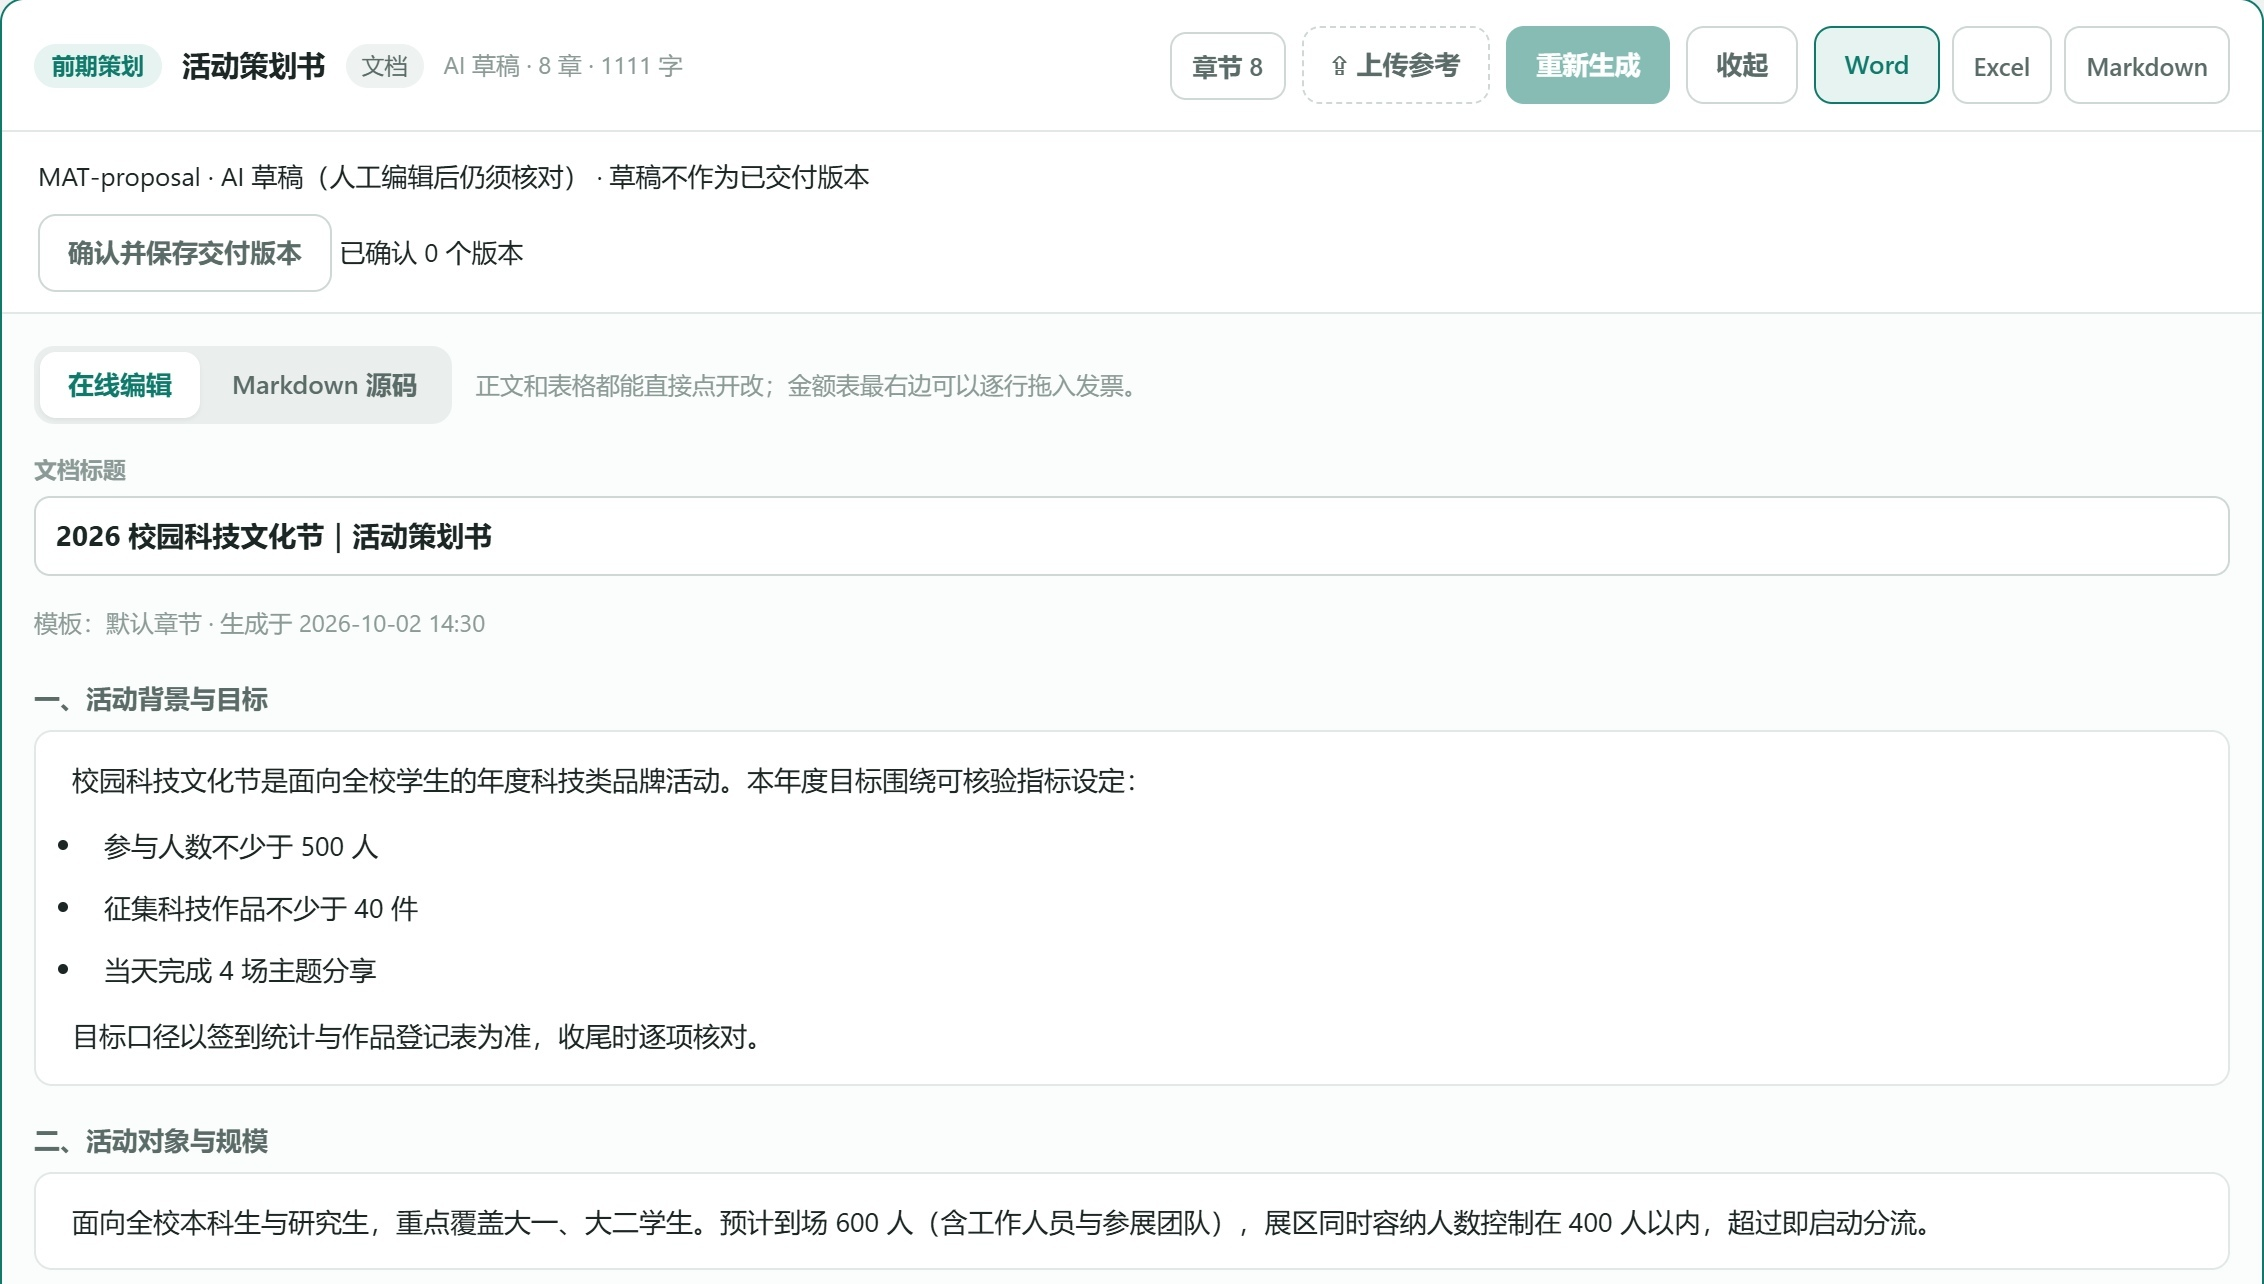
\includegraphics[width=\textwidth]{screenshots/material-edit-detail-d39138e.jpg}
\caption{策划书的正文编辑、版本确认与导出入口（局部）}
\label{fig:ui-material}
\end{figure}

宣传海报的提示词由项目事实、文案、视觉说明与追加要求装配，并保留手改稿。图\ref{fig:poster}依据活动名称、日期、地点和板块生成，使用墨绿色与白底风格；主文案逐项核对后用于报告展示。\source{7}

\begin{figure}[H]\centering

\includegraphics[width=0.38\textwidth]{poster-campus-tech-festival.png}
\caption{依据项目事实生成的校园科技文化节宣传海报}
\label{fig:poster}
\end{figure}

AI辅助展开和生成，小组核对事实、结构与执行条件，完成修订、确认和归档，使生成内容成为有依据的活动材料。

\subsection{建设过程与成员分工}
建设按“结构搭建、材料完善、协作闭环”推进：10月2日至5日形成四阶段原型、信息录入、材料编辑导出与扫码收集；随后扩展自定义产出、知识引用和卡片依赖，10月10日至11日连接共享、账号、人员轮班与版本交付。每轮按 PDCA 实现、检查、修订并留档，Git和开发记录保存改动及验证结果。\source{5,7}

小组围绕工作台制作、报告与展示、测试核查、流程与风险梳理开展协作，具体分工见表\ref{tab:members}。跨模块修改先对齐字段和输出，再整合检查。

\begin{table}[H]\centering\small
\caption{小组成员与分工}
\label{tab:members}
\begin{tabularx}{\textwidth}{L{4cm}Y}
\toprule
成员（学号） & 负责内容 \\
\midrule
张敬宇（2024303784） & 工作台整体设计与功能制作及测试，报告撰写与 PPT 内容整理。 \\
刘秋彤（2024303785） & 工作台界面与交互制作及完善，报告撰写及PPT 编排及材料整合。 \\
王梓安（2024303777） & 功能测试、操作核查与问题记录。 \\
胡辰凯（2024303779） & 活动流程与风险预案梳理、材料核对。 \\
\bottomrule
\end{tabularx}
\end{table}

\section{应用成果与测试验证}
\subsection{全周期应用成果}
校园科技文化节项目将活动事实与任务、资源、材料关联，初始项目包包含27项任务、19项风险、9项资源、3项知识素材和2条演练记录。成果按 MECE 过程时间法组织，覆盖策划、宣传、执行和收尾材料，并以“内容齐全、口径一致、行动可落实”核验。\source{8}

\textbf{任务闭环以实际交付为依据}：实名责任人提交经确认的材料版本，组织者验收后推进状态；班次与考勤记录执行过程。图\ref{fig:delivery}将 5W2H 的责任、成果、时间与行动落实到交付流程，历史验收始终绑定原版本。\source{5}

\begin{figure}[H]\centering
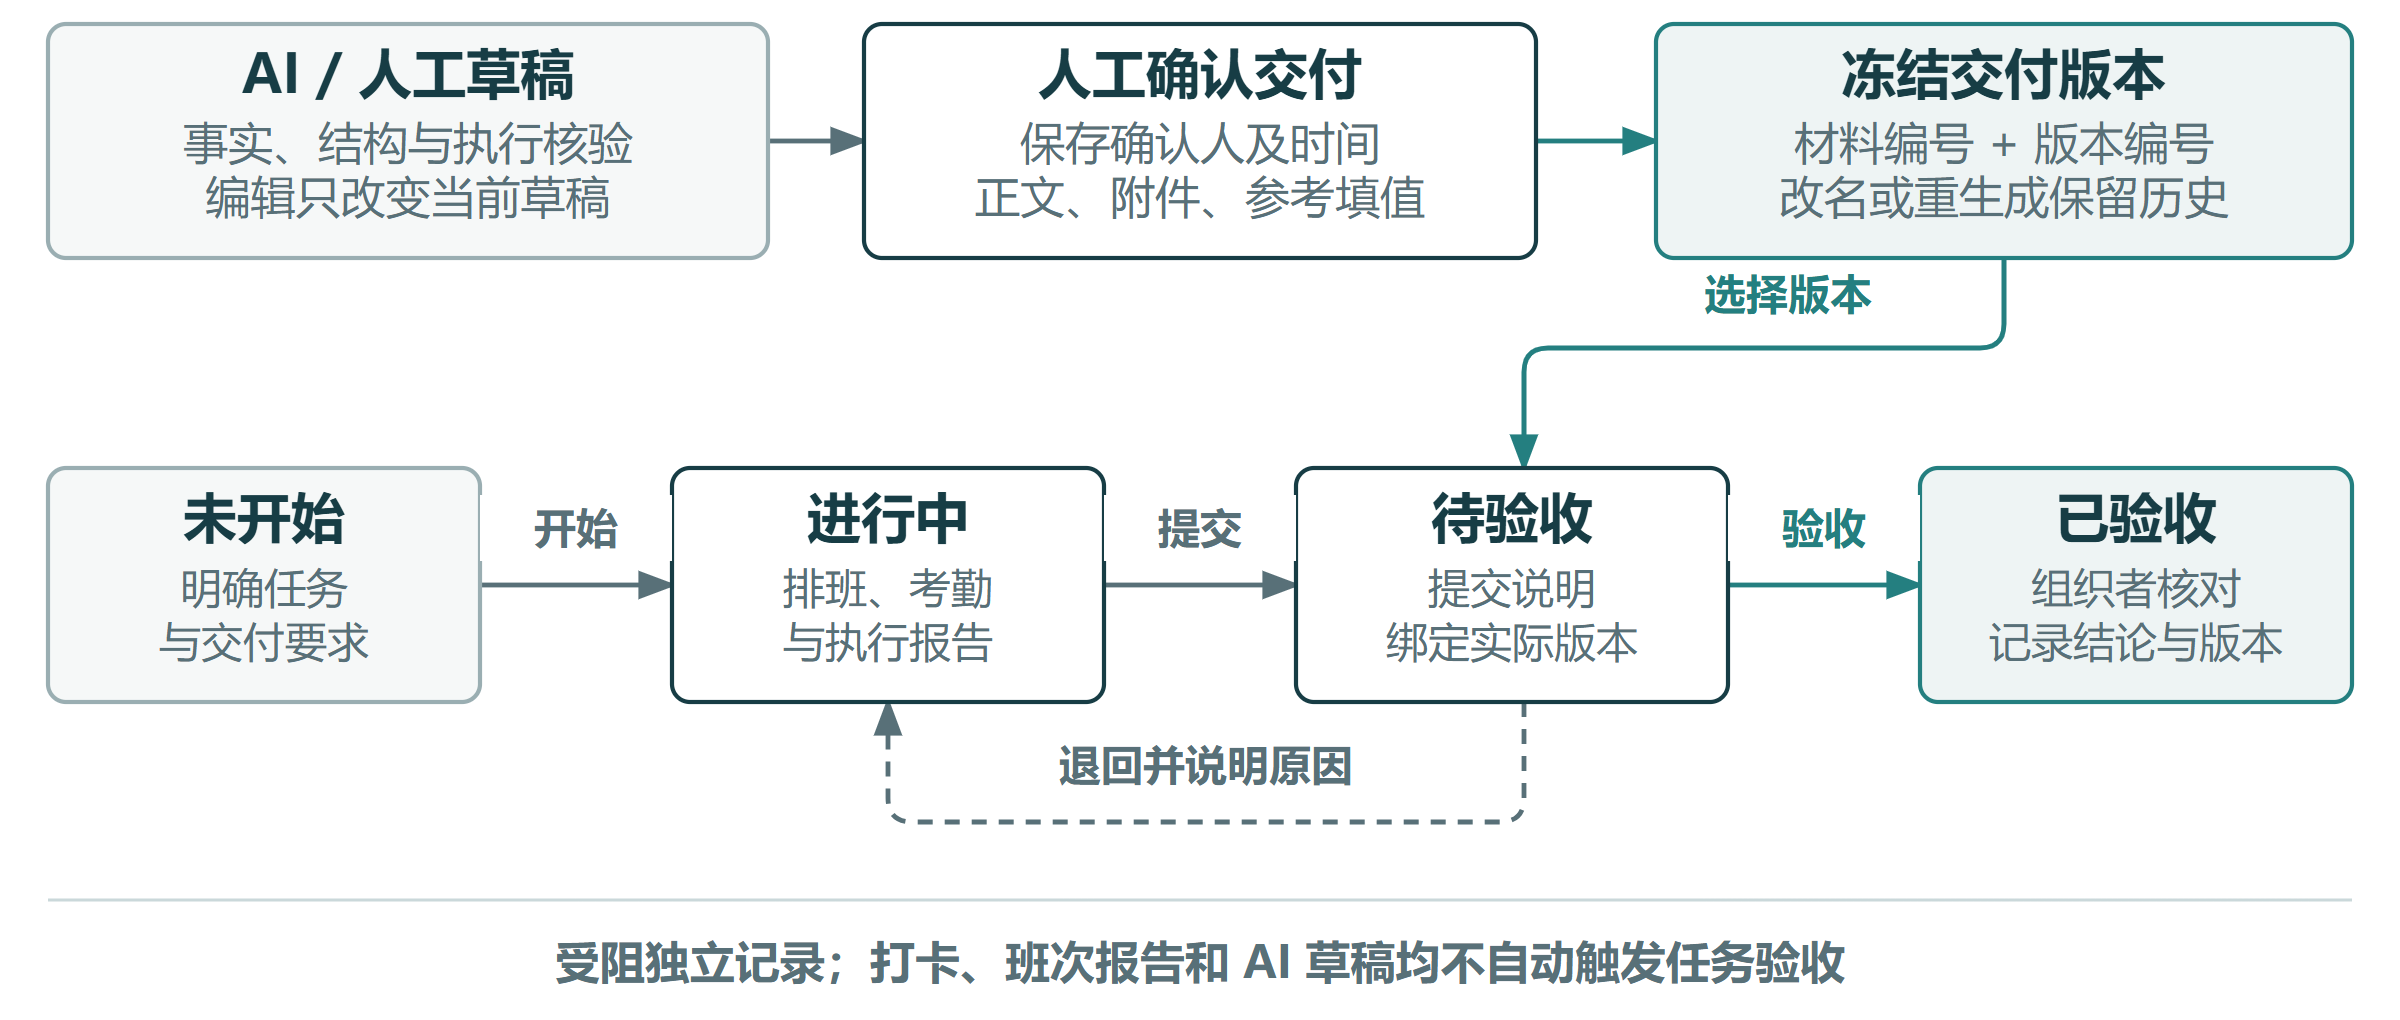
\includegraphics[width=\textwidth]{task-delivery-flow.png}
\caption{任务状态、交付版本与人工验收的关联}
\label{fig:delivery}
\end{figure}

风险应用以恶劣天气为例，可能性4、影响4，评分16，列为高风险。图\ref{fig:weather}明确准备、决策、行动与升级路径，落实 PDCA 的预案、推演、复核与修订。场地启用及应急决策由组织者确认。\source{8}

\begin{figure}[H]\centering
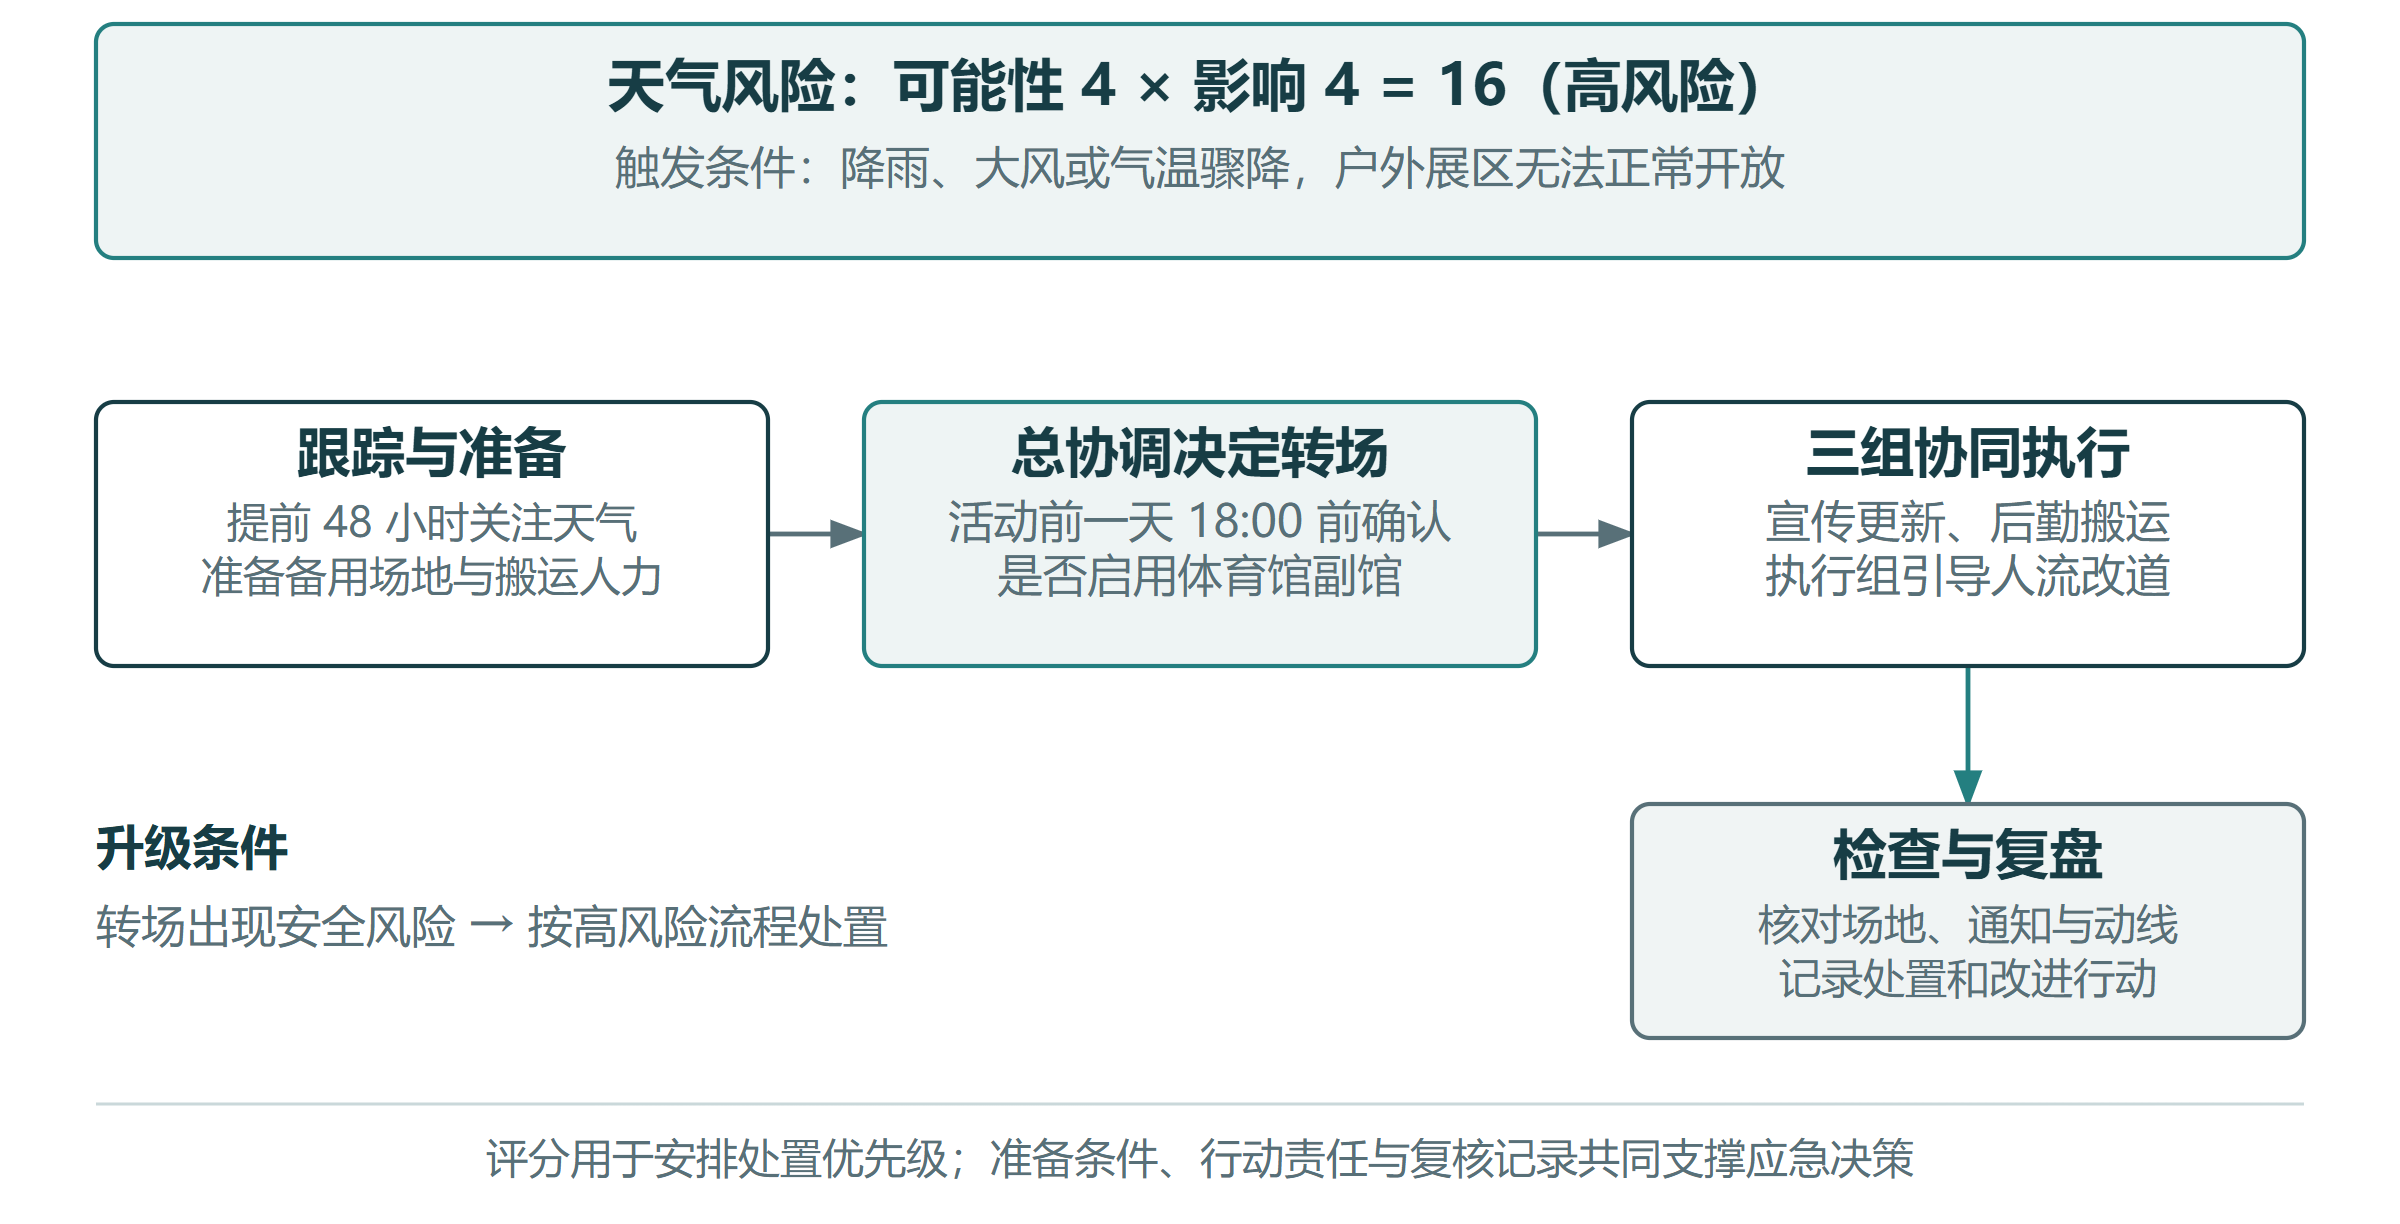
\includegraphics[width=\textwidth]{weather-response.png}
\caption{天气风险从识别、准备到响应与复核的路径}
\label{fig:weather}
\end{figure}

\subsection{测试验证与改进}
验证依据提交\texttt{d39138e}，使用本机服务、临时数据及独立角色会话。按“目标—规则—正常与反例—证据”构建逻辑树（图\ref{fig:validation}），检查结构完整、数据一致、权限正确与操作可恢复。AI交互采用受控响应核对引用和写回；策划书与海报另行人工核验事实、结构与文案。\source{9}

\begin{figure}[H]\centering
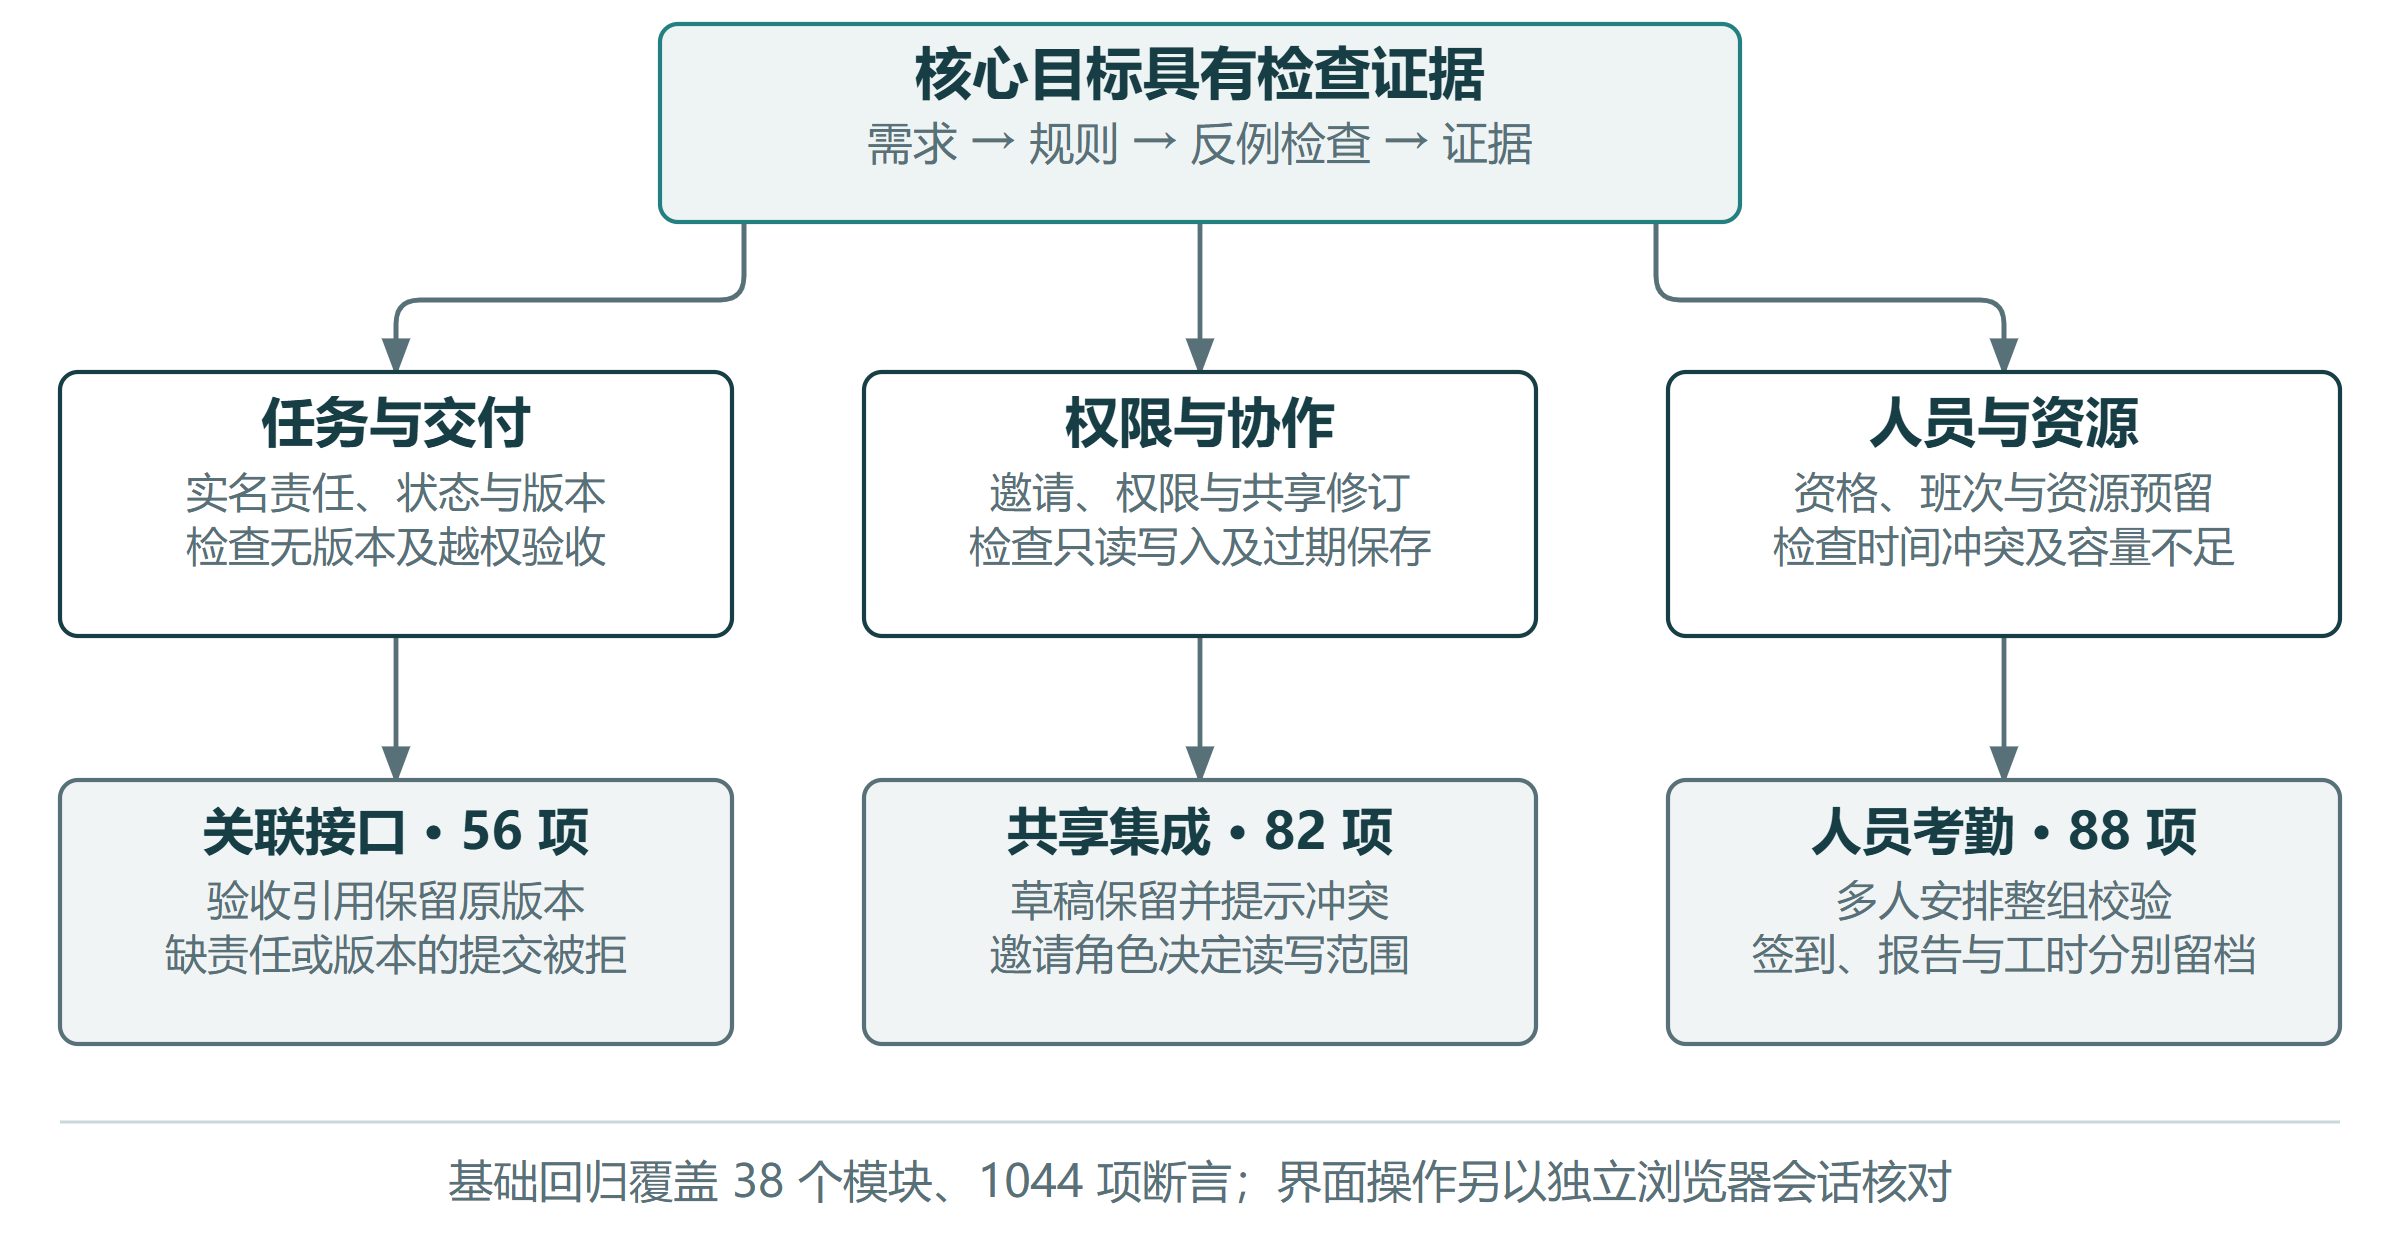
\includegraphics[width=\textwidth]{validation-evidence.png}
\caption{从目标、规则到反例与验证证据的逻辑树}
\label{fig:validation}
\end{figure}

\begin{table}[H]\centering\small
\caption{验证范围与本次运行结果}
\label{tab:tests}
\begin{tabularx}{\textwidth}{L{2.6cm}Y L{2.6cm}}
\toprule
验证组 & 主要检查内容 & 运行结果 \\
\midrule
离线基础回归 & 38个模块；结构、计算、导出与存档 & 1044项断言，失败0项 \\
共享与考勤 & 权限、保存冲突、重复提交与恢复 & 82项通过 \\
人员与排班 & 账号、授权、轮班冲突及资源校验 & 88项通过 \\
任务交付关联 & 实名责任、版本引用、提交与验收 & 76项通过 \\
浏览器交互 & 多角色与手机入口、引用及材料写回 & 133项通过 \\
\bottomrule
\end{tabularx}
\end{table}

各组检查均通过，任务关联组的76项包含56项接口检查和20项浏览器检查。复测确认：材料更新不改变既有验收引用，只读写入与过期覆盖被拒绝，排班冲突或资源不足时整组保存失败。\source{9}

改进遵循 PDCA，以“问题—原因—修改—复测”闭环推进，重点完善实名责任、版本快照和冲突保护。图\ref{fig:task-evidence-ui}展示执行记录与交付验收分别核验：班次结束、报告提交后，整项任务仍须补齐责任和交付证据，再由组织者验收。\source{5,7,9}

\begin{figure}[H]\centering
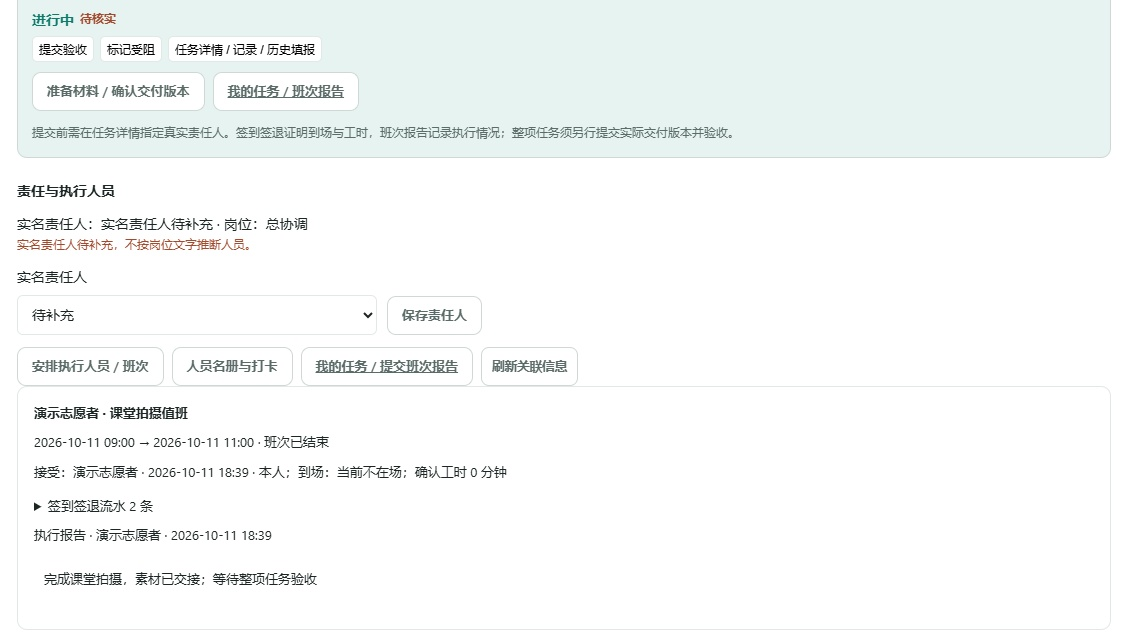
\includegraphics[width=\textwidth]{screenshots/task-delivery-detail.jpg}
\caption{班次记录与整项交付验收分别核验（演示会话局部）}
\label{fig:task-evidence-ui}
\end{figure}

\section{总结与思考}
\subsection{项目成果与方法价值}
项目围绕三个核心目标形成了相互关联的能力。全周期管理把策划、筹备、执行和收尾连接起来，以任务、责任、期限和检查点跟踪推进；中间产物依托统一事实、知识引用和技能包生成，经编辑、版本确认与导出形成可检查成果；风险管理把评分、触发条件、预防、响应和升级路径落实到台账、处置卡和变更演练。

结构化思维贯穿了需求、设计、AI使用与验证。表\ref{tab:method-value}将方法对应到具体设计选择及证据，说明其价值如何落在工作台的操作中。

\begin{table}[H]\centering\small
\caption{结构化方法、设计选择与检查证据的对应}
\label{tab:method-value}
\begin{tabularx}{\textwidth}{L{2.2cm}Y Y}
\toprule
方法 & 对设计与判断的影响 & 对应证据 \\
\midrule
SPIN & 从活动组织难点推导统一信息、责任与材料需求 & 背景、难点、影响和需求分析 \\
MECE与逻辑树 & 按时间拆解四阶段，按对象区分任务、人员、材料与风险 & 任务树、需求追踪表和验证逻辑树 \\
5W2H & 把任务细化为人员、时间地点、动作、资源与交付 & 实名责任、人员班次、资源预留和版本引用 \\
SWOT与方案比较 & 同时考虑目标覆盖、已有能力和实施条件 & 路线比较、风险应对与技术选择理由 \\
ALIGN与RTGO & 把用途、依据、事实边界及输出形式写入输入契约 & 技能包、引用资料、卡片依赖和人工修订 \\
PDCA & 用检查结论决定修订与下一轮行动 & 预案演练、验收退回、问题复测与改进记录 \\
\bottomrule
\end{tabularx}
\end{table}

项目也明确了人机分工。使用者定义目标、约束和验收标准，AI辅助整理信息、展开方案与生成文字图像；小组负责比较路线、核对事实、修订材料和整合成果。遇到缺项时先补充依据，遇到冲突时先明确规则，遇到验收争议时回查具体版本。这样，AI输出进入可追踪的工作过程，判断依据与责任仍有清楚的归属。

\Needspace{0.40\textheight}
\section*{参考资料}
\begingroup\small
\begin{enumerate}[label={[\arabic*]},leftmargin=2.5em,itemsep=3pt]
\item 课程《“结构化思维”大作业要求》：选题四、统一提交物及课堂汇报要求。
\item 课程《第1章 AIGC与结构化思维概述》：引导案例“全链路多模态作品”。
\item 课程《第2章 结构化思维核心框架与基础工具》：2.1.2逻辑树，2.2.1 MECE，2.2.5 SPIN，2.3.1 SWOT，2.3.2 5W2H，2.3.4 PDCA，2.4三维组织法，2.5人机分工。
\item 课程《0929提示词工程基础》PPT：第28页 ALIGN、第32页 RTGO；配套课堂演示手册。
\item 项目仓库提交 \texttt{d39138e}：README、账号与共享代码、《多人共享与考勤验收》《服务人员账号与统一资源管理》，以及任务生命周期和交付版本实现。
\item 同一提交：《知识库与素材库搭建指南》及对应资料管理代码。
\item 同一提交：《迭代进度记录》，含海报提示词装配、图像生成与手改优先的开发及验证记录。
\item 同一提交：活动策划书、风险台账、复盘报告等技能包、产出注册表及校园科技文化节示例项目包。
\item 2026年10月11日验证记录：该提交的离线回归、共享集成、人员账号、任务交付关联及浏览器综合检查；采用本机服务、临时数据与独立会话。
\end{enumerate}

\endgroup
\end{document}
